\documentclass{book}
\usepackage[margin=1.5in]{geometry} 
\usepackage[spanish]{babel}
\usepackage{sectsty}
\usepackage{amsmath,amsthm,amssymb,hyperref,braket,fontspec,color, graphicx, appendix, empheq, subfig}
\usepackage[dvipsnames]{xcolor}
\setromanfont[
BoldFont=QuattrocentoSans-Bold.ttf, 
ItalicFont=QuattrocentoSans-BoldItalic.ttf,
BoldItalicFont=QuattrocentoSans-Italic.ttf
]{QuattrocentoSans-Regular.ttf}
\setsansfont[
BoldFont=QuattrocentoSans-Bold.ttf,
ItalicFont=QuattrocentoSans-BoldItalic.ttf,
BoldItalicFont=QuattrocentoSans-Italic.ttf
]{QuattrocentoSans-Regular.ttf}
\begin{document}
\author{\textcolor{Red}{Raúl Coto Cabrera, Bing He, Daniel Castillo Castro}}
\title{\textcolor{Red}{Métodos Matemáticos de la Óptica Cuántica}}
\vspace{0.05in}
\chapterfont{\color{Red}}
\sectionfont{\color{Red}}
\subsectionfont{\color{Red}}
\everymath{\color{blue}}
\everydisplay{\color{blue}}
\maketitle
\tableofcontents
\chapter{Introducción}
El siguiente apunte es una transcripción de actividades realizadas durante la asignatura "Métodos Matemáticos de la Óptica Cuántica" del programa de Doctorado en Física con mención en Óptica e Información Cuántica de la Universidad Mayor, Impartido por los profesores Raúl Coto Cabrera (Quién desarrolló los primeros capítulos) y Bing He (Quién desarrolló el último capitulo correspondiente a Ruido Cuántico). \\


En la literatura existen pocos libros en español dedicados a un área incipiente de la Física como son los \textcolor{red}{Sistemas Cuánticos Abiertos}. Como es conocido por los estudiantes de ciencias, la ecuación fundamental de la dinámica de sistemas cuánticos es la Ecuación de Schrodinger, que es una ecuación diferencial de orden matricial. Esta ecuación tiene como problema que corresponde a un modelo simplificado de la Física a nivel Cuántico, que funciona bien para sistemas aíslados de su ambiente, pero falla al considerar sus posibles efectos.\\


\begin{figure}[ht]
\centering
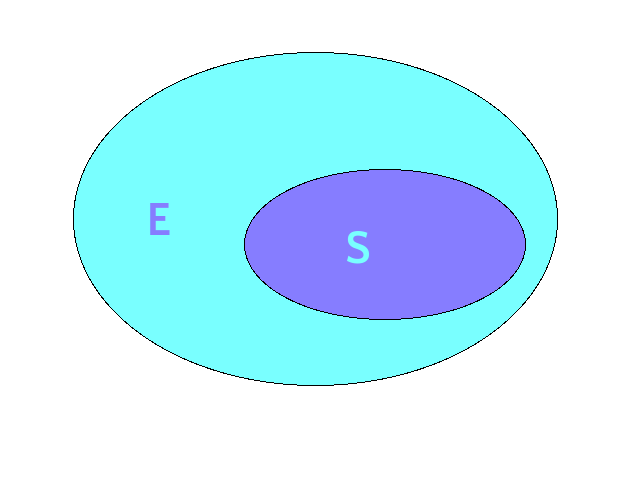
\includegraphics[width=0.55\textwidth]{qos.png}
\caption{Representación pictórica de un sistema cuántico abierto $S$, que tiene su propia dinámica, que puede ser descrita por una ecuación de Schrodinger. Sin embargo, al considerar el ambiente (descrito aquí como $E$) se requerirán nuevos métodos. Nótese que no hay reglas para separar a $S$ de $E$, la elección de dicha separación es arbitraria, por lo que e puede elegir de forma adecuada para simplificar el problema.}
\end{figure}

Agregar al ambiente en un sistema puede complejizar considerablemente el planteo del problema. Esto ha llevado al desarrollo de nuevos métodos matemáticos para resolver estos problemas, que son típicas en sistemas físicos observados en Óptica en Información Cuántica. Esto explica su necesidad en programas de posgrado vinculadas a dicho campo de investigación.

\begin{figure}[ht]
\centering
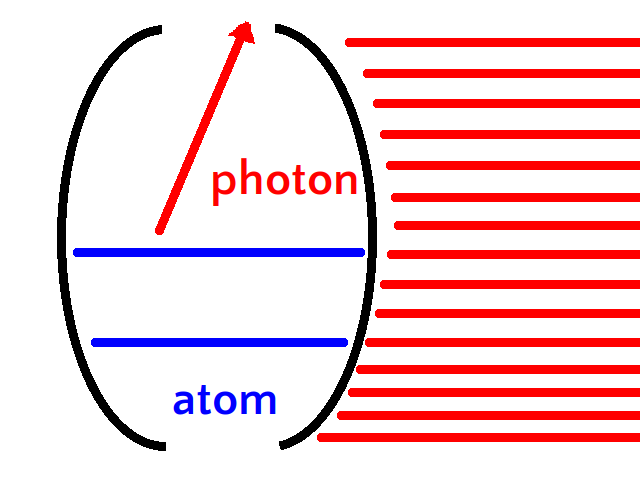
\includegraphics[width=0.6\textwidth]{cav.png}
\caption{Representación de un sistema óptico simple que se puede considerar un sistema cuántico abierto. Cumple el rol de $S$ un átomo de 2 niveles presente en una cavidad, mientral que el de $E$ lo cumple el campo magnético que rodea a dicha cavidad. Se busca estudiar el efecto que tiene el campo en los electrones del átomo, que pueden producir emisión estimulada de fotones. }
\end{figure}
En este libro se explorará en primera instancia el sentido y limitantes de la ecuación de Schrodinger. Luego de introducirá el concepto de \textcolor{red}{Ecuación Maestra}, posible de derivar de manera fenomenológica o a partir de principios fundamentales (lo que se ejemplificará usando el Modelo de Spin Bosónico). \\

Otro método consiste básicamente en añadir elementos estocásticos a la ecuación de Schrodinger. Dicho método es conocido como \textcolor{red}{Quantum Jumps}. Se ejemplifica la ejecución de dicho método en el modelo Jaynes-Cummings.\\

Un tercer método posible de usar es la descripción del sistema físico en \textcolor{red}{Espacio de Fases}, lo que convierte ecuaciones diferenciales matriciales en ecuaciones diferenciales algebraicas. Se ejemplificará el método para condensados Bose-Einstein.\\

El libro concluye con otra forma de entender los efectos del ambiente: como \textcolor{red}{Ruido Cuántico} que afecta al sistema cerrado a estudiar. Se introduce el análisis de Langevin que parte de esta consideración, y se demuestra que usando ruido se puede entender la ecuación maestra de forma más intuitiva.
\chapter{Ecuación de Schrodinger}
 Evolución temporal unitaria para funciones de onda. Solo para sistemas cerrados, no se le puede escapar información. Las condiciones de borde generan ondas estacionarias, las que fijan modos.
En el hamiltoniano del sistema se genera un elemento de Hoping con la forma:
\begin{equation}
    \label{eq2.1} J(a_1^\dag a_2+a_2^\dag a_1) 
\end{equation}
Dicho elemento produce un efecto túnel, que lleva a una onda evanescente a una misma frecuencia $\omega$. Esto es llamado \textcolor{red}{coherent scattering}, lo que explica la emisión estimulada. En efecto, lo que se está haciendo es acoplar niveles atómicos. El hamiltoniano para el sistema total es:
\begin{equation} \begin{aligned}
   \label{eq2.2} H=\omega_0 \sigma_{ee} +\omega_c a^\dag a + g(\sigma^++\sigma^-)(a^\dag a)+\sum_{i=0}\omega_i c_i^\dag c_i\\ +\sum_{i=0}G_i(\sigma^++\sigma^-)(c_i^\dag+c_i)+\sum_{i=0}G_i^* \sigma_z (c_i^\dag +c_i)+\sum_{i=0} k_i(a^\dag+a)(c_i^\dag+c_i)
\end{aligned} \end{equation}
Los sumandos del hamiltoniano corresponde al campo libre, al modelo de Rabi (acoplamiento campo materia, superconductor), el reservorio libre y las interacciones de resonancia con el campo y la cavidad respectivamente. \\

Si para \ref{eq2.2} $\omega_0>>g$, se produce lo llamado \textcolor{red}{Acoplamiento Débil}, obteniéndose el hamiltoniano \textcolor{red}{Jaynes-Cumming}. Otro comentario es que el sistema debe modelar pérdidas para tener significado físico y coherencia con los resultados experimentales. De acuerdo a lo dicho en el capítulo anterior, el sistema se puede \textit{cerrar} el sistema donde se desee, con una sola condición: el hamiltoniano del sistema debe tener la fórmula:

\begin{equation} \label{eq2.3} H=H_S+H_R+H_{SR}\end{equation}
Dicho hamiltoniano debe cumplir, en principio con la Ecuación de Schrodinger:
\begin{equation}\label{eq2.4} i\hslash \frac{\partial}{\partial t} \ket{\phi(t)}=H(t)\ket{\phi(t)}\end{equation}
Para un sistema cerrado esta ecuación \textcolor{red}{siempre se cumple}.
\section{Evolución temporal como operación unitaria}
Una forma de observar la evolución temporal producida por \ref{eq2.4} es integrarla para un intervalo de tiempo entre $t_0$ y $t$
\begin{equation}\label{eq2.5}\ket{\phi(t)}=U(t,t_0)\ket{\phi(t_0)}\textcolor{red}{\Rightarrow} i \hslash \frac{\partial}{\partial t}U(t,t_0)=H(t)U(t,t_0)\end{equation}
Lo que implica que para una función de onda normalizada la evolución temporal se puede considerar una \textcolor{red}{Transformación Unitaria}, lo que implica que la operación se puede revertir en el tiempo.\\

El hecho de que la operación se pueda revertir es algo de importancia fundamental, ya que define que el sistema es \textcolor{red}{Markoviano}, lo que se define como un sistema que no tiene memoria, es decir, cuya evolución en un intervalo anterior solo depende del intervalo inmediatamente anterior. \\

El operador $U(t,t_0)$ tiene como solución:
\begin{equation}\label{eq2.6}U(t,t_0)=T_{\leftarrow}e^{\frac{-i}{\hslash}\int_0^t H(s)ds}\end{equation}
Este operador es llamado una \textcolor{red}{Integral Ordenada}, lo que significa que es una integral anidada cuyos valores de integración van de menor a mayor, es decir:
\begin{equation}\label{eq2.7}t_1<t_2<t_3...<t_n \textcolor{red}{\Rightarrow} T_{\leftarrow}\int_0^t=\int_0^{t_n}...\int_0^{t_2}\int_0^{t_1}\end{equation}
\subsection{{Forma del operador evolución temporal}}
El operador expresado anteriormente puede escribirse de forma más manejable. Tomando la ecuación de \ref{eq2.5}
\begin{equation}\label{eq2.8}\dot{U}(t,t_0)=-\frac{i}{\hslash}H(t)U(t,t_0)\end{equation} Integrando \ref{eq2.8} y usando la propiedad $U(t_0,t_0)=\mathbb{I}$
\begin{equation}\label{eq2.9}U(t,t_0)=\mathbb{I}-\frac{i}{\hslash}\int_0^t H(t_1)U(t_1,t_0)dt_1\end{equation} Si se aplica recursivamente \ref{eq2.9} para $U(t_1,t_0)$ en el mismo \ref{eq2.9}
\begin{equation}\label{eq2.10} U(t,t_0)=\mathbb{I}-\frac{i}{\hslash}\int_0^tH(t_1)(\mathbb{I}-\frac{i}{\hslash}\int_0^{t_1} H(t_2)U(t_2,t_0) dt_2)dt_1\end{equation}
Si lo anterior se repite varias veces se obtiene finalmente una sumatoria infinita de la forma:
\begin{equation}\label{eq2.11}U(t,t_0)=\mathbb{I}-\frac{i}{\hslash}\int_0^t H(t_1) dt_1+(-\frac{i}{\hslash})^2\int_0^t\int_0^{t_1} H(t_1)H(t_2)dt_1dt_2 + ...\end{equation}
Si $[H(t_i),H(t_j)]=0 \forall t_i,t_j$ \ref{eq2.11} se simplifica: \begin{equation}\label{eq2.12}U(t,t_0)=\sum_k \frac{1}{k!}(\frac{-i}{\hslash})^k (\int_0^tH(s)ds)^k=e^{-\frac{i}{\hslash}\int_0^s H(s)ds}\end{equation}
Y si H es una constante, \ref{eq2.12} se simplifica más aún:
\begin{equation}U(t,t_0)=e^{\frac{-i}{\hslash}Ht}\end{equation}
\subsection{{Exponencial temporal como producto infinito}}
El operador de \ref{eq2.7} se puede escribir en otras formas: Para un intervalo entre $t_0$ y $t$ se pueden definir $N$ intervalos de largo  infinitesimal $\Delta t$.
\begin{equation} \label{eq2.14} t_i= t_0\cdot i\Delta t: t_{N+1}=t\end{equation}
Integrando \ref{eq2.8} en un intervalo entre $t_i$ y $t_{i+1}$ 
\begin{equation}\label{eq2.15}U(t_{i+1},t_0)-U(t_i,t_0)=-\frac{i}{\hslash}H(t_i)\Delta t U(t_i,t_0)=(\mathbb{I}-\frac{i}{\hbar}H(t_i)\Delta t)U(t_i,t_0)\end{equation}
Aplicando \ref{eq2.15} para el intervalo de \ref{eq2.14}
\begin{equation}\label{eq2.16}\begin{aligned}U(t,t_0)=(\mathbb{I}-\frac{i}{\hbar}H(t_N)\Delta t)U(t_N,t_0) \\ (\mathbb{I}-\frac{i}{\hbar}H(t_N)\Delta t)(\mathbb{I}-\frac{i}{\hbar}H(t_{N-1})\Delta t)U(t_{N-1},t_0)\end{aligned}\end{equation}
Entonces, aplicando repetidas veces el procedimiento de \ref{eq2.16}
\begin{equation}\label{eq2.17}U(t,t_0)=\prod_{i=1}^N U(t_i,t_0)\end{equation}
\subsection{Propiedades del operador Evolución}
Usando la definición del operador evolución de \ref{eq2.17} se puede demostrar de forma más simple algunas propiedades. Para evolucionar en 2 intervalos que están juntos:
\begin{equation}\label{eq2.18}t_1=t_0+N\Delta t, t_2=t_1+M\Delta t= t_0+(N+M)\Delta t\end{equation}
Se cumple que:
\begin{equation}\label{eq2.19}U(t_2,t_0)=\prod_{i=1}^{N+M} U(t_i,t_0)=\prod_{i=1}^{N} U(t_i,t_0)\prod_{i=N+1}^{N+M} U(t_i,t_0)\end{equation}
Con lo que se demuestra que
\begin{equation}\label{eq2.20}U(t_2,t_0)=U(t_2,t_1)U(t_1,t_0)\end{equation}
Además, la inversa del operador evolución se puede obtener a partir  de \ref{eq2.20}
\begin{equation}\label{eq2.21}\mathbb{I}=U(t_0,t_0)=U(t_0,t)U(t,t_0) \textcolor{red}{\Rightarrow} U^{-1}(t,t_0)=U(t_0,t)\end{equation}
\section{Formas para hallar soluciones de la ecuación de Schrodinger}
La ecuación de Schrodinger puede resolverse de 2 modos para mostrar cómo funcionan ambos métodos se ejemplicarán con el hamiltioniano Jaynes-Cummings:
\subsection{Método de Diagonalización}
A partir de \ref{eq2.6}, se puede derivar la solución del sistema considerando commo truco escoger $\ket{\phi(t_0)}$ en una base donde el hamiltoniano sea diagonal, es decir, la base correspondiente a los autoestados del  hamiltoniano. El hamiltoniano de Jaynes Cumming es
\begin{equation}\label{eq2.22} H=\omega_a\sigma_{ee}+\omega_c aa^\dag +g(\sigma^+a+\sigma^-a^\dag)\end{equation}
Este tiene como autoestados los llamados \textit{estados vestidos} $\ket{n_+}$ y $\ket{n_-}$. El Hamiloniano opera en el espacio de Hilbert compuesto de un campo electromagnético representado por estados número y un átomo de 2 niveles representado por los estados $\ket{g}$ (por \textit{ground state}, el estado fundamental que es de menor energía) y $\ket{e}$ (por \textit{excitado}, el estado de mayor energía). Los estados vestidos se escriben en función de los estados compuestos de ambas bases (también llamados \textit{Estados Desnudos}:
\begin{equation}\label{eq2.23}\begin{aligned} \ket{n_-}=cos \theta_n\ket{n,g}-sin \theta_n\ket{n-1,e}\\\ket{n_+}=sin \theta_n\ket{n,g}+cos\theta_n\ket{n-1,e} \end{aligned}\end{equation}
Pudiéndose escribir el hamiltoniano del sistema como
\begin{equation}\label{eq2.24}H=\sum_{n=1}^N(E_{n+}\ket{n+}\bra{n+}+E_{n-}\ket{n-}\bra{n-}), (E_{n\pm}=\omega_c n+\frac{\Delta}{2}\pm\frac{1}{2}\sqrt{\Delta^4+4g^2n})\end{equation}
Y si se escribe la función de onda dependiente del tiempo como un estado inicial operado con un operador de Schrodinger:
\begin{equation}\label{eq2.25}\ket{\phi(t)}=e^{-\frac{i}{\hslash} Ht}\ket{\phi(0)}\end{equation}
Se puede aprovechar lo escrito en \ref{eq2.9} para escribir $\phi(0)$ en la base de estados vestidos y luego aplicar el hamiltoniano diagonalizado
\begin{equation}\label{eq2.26}\begin{pmatrix}\ket{n,g}\\ \ket{n-1,e}\end{pmatrix}=\begin{pmatrix}cos \theta_n&sin\theta_n\\-sin\theta_n&cos\theta_n\end{pmatrix}\begin{pmatrix}\ket{n_-}\\\ket{n_+}\end{pmatrix}\end{equation}
Notando que la transformación de estados es una rotación, \ref{eq2.26} es fácil de invertir
\begin{equation}\label{eq2.27}\begin{pmatrix}\ket{n_-}\\\ket{n_+}\end{pmatrix}=\begin{pmatrix}cos\theta_n&-sin\theta_n\\sin\theta_n&cos\theta_n\end{pmatrix}\begin{pmatrix}\ket{n,g}\\\ket{n-1,e}\end{pmatrix}\end{equation}
Por ejemplo, si se considera condición inicial $\ket{0,e}$, este estado en la base definida en \ref{eq2.23} es 
\begin{equation}\label{eq2.28}\ket{\phi(0)}=\ket{0,e}=-sin\theta_n\ket{1_-}+cos\theta_n\ket{1_+}\end{equation}
Aplicando \ref{eq2.25} 
\begin{equation}\label{eq2.29}\ket{\phi(t)}=e^{-\frac{i}{\hslash}Ht}(-sin\theta_n\ket{1_-}+cos\theta_n\ket{1_+})\end{equation}
Al ser el hamiltoniano diagonalizado, la evolución temporal se simplifica el resultado es
\begin{equation}\label{eq2.30}\ket{\phi(t)}=e^{-\frac{i}{\hslash}E_{n-}t}(-sin\theta_n\ket{n_-})+e^{-\frac{i}{\hslash}E_{n+}t}(cos\theta_n\ket{n_+})\end{equation}
\subsection{Método de Función de onda} Un método posible es el llamado \textcolor{red}{Método de función de onda}. Consiste en comenzar suponiendo que la solución de la ecuación de Schrodinger tiene la forma:
    \begin{equation}\label{eq2.31}\ket{\phi(t)}=\sum_i a_i(t)\ket{\phi_i}\end{equation}
    Insertando \ref{eq2.31} en \ref{eq2.4} resulta:
\begin{equation}\label{eq2.32}i\hslash\sum_i(\frac{\partial}{\partial t}a_i(t))\ket{\phi_i(t)}=H(t)\sum_i a_i(t)\ket{\phi_i}\end{equation}
Lo que define una ecuación para los $a_i(t)$
\begin{equation}\label{eq2.33}i\hslash\dot{a_i}=\sum_i a_i(t) \bra{\phi_i}H(t)\ket{\phi_i}\end{equation}
En el ejemplo de Jaynes-Cummings, el planteo de la forma de \ref{eq2.31} se vuelve:
\begin{equation}\label{eq2.34}\ket{\phi(t)}=a_+(t)\ket{n_+}+a_-(t)\ket{n_-}\end{equation}
y la ecuación de \ref{eq2.33} se aplica para $a_+$ y $a_-$:
\begin{equation}\label{eq2.35} \begin{aligned}i\hslash \dot{a}_+(t)=a_+(t)E_{n+}\textcolor{red}{\Rightarrow}a_+(t)=a_+(0)e^{-\frac{i}{\hslash}E_{n+}t}\\i\hslash \dot{a}_-(t)=a_-(t)E_{n-}\textcolor{red}{\Rightarrow}a_-(t)=a_-(0)e^{-\frac{i}{\hslash}E_{n-}t}\end{aligned}\end{equation}
Reemplazando en la solución de forma \ref{eq2.31} en lo obtenido en \ref{eq2.35}
\begin{equation}\label{eq2.36}\ket{\phi(t)}=a_+(0)e^{-\frac{i}{\hslash}E_{n+}t}\ket{n_+}+a_-(0)e^{-\frac{i}{\hslash}E_{n-}t}\ket{n_-}\end{equation}
Si se fija como condición inicial$\ket{0,e}$
\begin{equation}\label{eq2.37}\ket{\phi(0)}=-sin\theta_n\ket{1_-}+cos\theta_n\ket{1_+}\textcolor{red}{\Rightarrow} a_-(0)=-sin\theta_n,a_+(0)=cos\theta_n\end{equation}
Por lo que la solución finalmente queda:
\begin{equation}\label{eq2.38}
\ket{\phi(t)}=e^{-\frac{i}{\hslash}E_{n+}t}(cos\theta_n\ket{n_+})+e^{-\frac{i}{\hslash}E_{n-}t}(-sin\theta_n\ket{n_-})\end{equation}
Nótese que la solución en \ref{eq2.38} es la misma de \ref{eq2.30} lo que demuestra que ambos métodos son equivalentes.
\chapter{Ecuación Maestra Fenomenológica}
Lo visto anteriormente es válido para sistemas cuánticos cerrados, que son más simples pero menos realistas (aunque funcionan adecuadamente como modelo en algunos casos). Para poder incluir sistemas abiertos, se necesita un método más general. Y allí surge la \textcolor{red}{Ecuación Maestra}, que no es más que una ecuacion diferencial  \textcolor{red}{matricial}.\\

Para un sistema cerrado o abierto siempre se puede encontrar una \textcolor{red}{matriz densidad} $\rho$, a la que siempre se le encontrará una posible descomposición espectral:
\begin{equation}\label{eq3.A}\rho=\sum_{ij}a_{ij}\ket{\phi_i}\bra{\phi_j}=\sum_\alpha \ket{\omega_\alpha}\bra{\omega_\alpha}\end{equation}
De manera análoga a los estados puros (los que se representan con vectores) se puede definir su respectivo operador evolución temṕoral:
\begin{equation}\label{eq3.B}\rho(t)=U(t,t_0)\rho(t_0)U^\dag(t,t_0)\end{equation}
Derivando temporalmente \ref{eq3.B} se obtiene:
\begin{equation}\label{eq3.C}\dot{\rho}(t)=\dot{U}(t,t_0)\rho(t_0)U(t,t_0)+U(t,t_0)\rho(t_0)\dot{U}^\dag(t,t_0)\end{equation}
Y usando la ecuación de Schrodinger para operadores de evolución en \ref{eq3.C}
\begin{equation}\label{eq3.D}\begin{aligned}\dot{\rho}(t)=-\frac{i}{\hslash} H(t)U(t,t_0)\rho(t_0)U^\dag(t,t_0)+\frac{i}{\hslash} U(t,t_0)\rho(t_0)U^\dag(t,t_0)H(t)\\ = \frac{-i}{\hslash}(H(t)\rho(t)-\rho(t)H(t)) \\ \textcolor{red}{\therefore} \dot{\rho}(t)=\frac{-i}{\hslash}[H(t),\rho(t)]\end{aligned}\end{equation}
La que es conocida en literatura como \textcolor{red}{Ecuación de Liouville} o \textcolor{red}{Ecuación de Von Neumann}.
Una forma conveniente de escribir esta ecuación es considerando la acción del conmutador como un \textcolor{red}{superoperador}, esto es, un operador que actúa tanto por derecha como por izquierda de $\rho(t)$
\begin{equation}\label{eq3.E}\dot{\rho(t)}=\mathcal{L}(t)[\rho(t)]\textcolor{red}{\Rightarrow} \rho(t)=[T_{\leftarrow}e^{\int_{0}^t \mathcal{L}(s) ds}]\rho(t_0)
\end{equation}
Lo que da a la evolución temporal de un estado una forma similar a la ecuación de Schrodinger. En estos sistemas nos interesa por lo general solo la evolución temporal del sistema, observando solo los efectos que el ambiente produce en él. Esto lleva a la \textcolor{red}{Ecuación Maestra}, que consiste en trazar sobre el ambiente la ecuación de Von Neumann.\\

Lo anterior puede hacerse de varias maneras. En este capítulo se abordará el enfoque fenomenológico para obtener ecuaciones maestras, esto es, a partir de suposiciones sobre el sistema. Se hará a partir de 2 métodos: Uno más formal matemático a partir de semigrupos, y uno más \textit{físico} que surge de considerar un sistema simple, método basado en el mostrado en \cite{Orszag}
\section{Derivación formal: semigrupos}
Comenzando con la evolución temporal de $\rho_A(t)$, parte A de una matriz compuesta $\rho_{AB}$
\begin{equation}\label{eq3.1}\rho_A(t)=tr_B{U(t,t_0)\rho(t_0)U^\dag(t,t_0)}\end{equation}
y la ecuación de Von Neumann 
\begin{equation}\label{eq3.2}\dot{\rho_A}(t)=-iTr_B[H(t),\rho(t)]\end{equation}
Se puede definir un \textcolor{Red}{mapa dinámico} como una función que va del espacio de Hilbert de A hasta sí mismo y consiste en \textcolor{Red}{superoperadores} que representan la evolución temporal para la matriz densidad para $\rho_B$ y tiempo fijos.
\begin{equation}\label{eq3.3}V(t):\mathbb{H}_A\textcolor{red}{\Rightarrow}\mathbb{H}_A\textcolor{red}{\Rightarrow} \rho_A(t)=V(t)\rho_A(0)=U(t,0)[\rho_A(0)\otimes\rho_B(0)]U^\dag(t,0) \end{equation}
Si se escribe $\rho_A$ en su base espectral, y se escribe las componentes matriciales del operador unitario $U(t,0)$ presente en \textcolor{blue}{\ref{eq3.3}} en la misma base:
\begin{equation}\label{eq3.4}\rho_A=\sum_\alpha\lambda_\alpha\ket{\varphi_\alpha}\bra{\varphi_\alpha}, W_{\alpha\beta}=\sqrt{\lambda_\alpha\lambda_\beta}\bra{\varphi_\alpha}U(t,0)\ket{\varphi_\beta}\end{equation}
Se puede reescribir la evolución temporal $V(t)$ como una medición generalizada (POVM)
\begin{equation}\label{eq3.5}V(t)\rho_A=\sum_{\alpha\beta}W_{\alpha\beta}(t)\rho_AW^\dag_{\alpha\beta}(t)\end{equation}
Dicha evolución temporal cumple como propiedades
\begin{equation}\label{eq3.6} \sum_{\alpha\beta}W_{\alpha\beta}^\dag(t)W_{\alpha\beta}(t)=\mathbb{I}_A\textcolor{red}{\Rightarrow} tr_A(V(t)\rho_A)=tr_A(\rho_A)=1\end{equation}
De acá se deduce que la operación evolución temporal cuántica es convexa, positiva y preservadora de traza, por lo que mantiene el sentido físico de las matrices densidad, que son las probabilidades. Estos operadores de evolución son los que forman un semigrupo que cumple con la siguiente propiedad fundamental.
\begin{equation}\label{eq3.7}V(t_1)V(t_2)=V(t_1+t_2) \end{equation}
La propiedad en \textcolor{blue}{\ref{eq3.7}} está vinculada con la Markovialidad.
Se define entonces un \textcolor{Red}{generador de semigrupo}, que consiste en un mapa lineal.
\begin{equation}\label{eq3.8}\mathcal{L}:V(t)=e^{\mathcal{L}t}\textcolor{red}{\Rightarrow} \dot{\rho_A(t)}=\dot{V}(t)\rho_A=\mathcal{L}\rho_A(t)\end{equation}
Se pretenderá entonces, construir el $\mathcal{L}$ más general en el espacio $\mathbb{H}_A\otimes\mathbb{H}_A$ definiendo operadores $F_i$ desde $0$ hasta $N^2$ definiendo un producto escalar para operadores
\begin{equation}\label{eq3.9}  X\cdot Y=Tr_A(X^\dag Y)\end{equation}
Se puede escribir el operador de medida generalizada, y por lo tanto el operador de evolución temporal como combinación lineal de los elementos de la base (considerando el producto escalar anterior:
\begin{equation}\label{eq3.10}W_{\alpha\beta}=\sum_{i=1}^{N^2} F_i(F_i\cdot W_{\alpha\beta}(t))\textcolor{red}{\Rightarrow} V(t)\rho_A=\sum_{\alpha\beta}\sum_{i,j=1}^{N^2} F_i(F_i\cdot W_{\alpha\beta}(t))\rho_AF_j^\dag(F_j\cdot W_{\alpha\beta}(t))^*\end{equation}
Llamando $c_{ij}$ a los resultados de los productos escalares la expansión de \textcolor{blue}{\ref{eq3.10}} se simplifica
\begin{equation}\label{eq3.11}c_{ij}=(F_i\cdot W_{\alpha\beta}(t))(F_j W_{\alpha\beta}(t))^*\textcolor{red}{\Rightarrow} V(t)\rho_A=\sum_{i,j}^{N^2}c_{ij}(t)F_i\rho_AF_j^\dag\end{equation}
Por la forma dada en la definición en \textcolor{blue}{\ref{eq3.11}}, los $c_{ij}$, forman una matriz hermítica y positiva.
Sin perder generalidad se define que el último operador de la lista sera proporcional a la identidad, así como que los operadores traza tendrán traza $0$
\begin{equation}\label{eq3.12}\forall i:[0,n^2-1] Tr_A F_i=0, F_{N^2}=\frac{\mathbb{I}_A}{\sqrt{N}}\end{equation}
Dicho esto se procede a evaluar la derivada de la evolución temporal, considerando \textcolor{blue}{\ref{eq3.8}}, la definición formal de derivada (con un tiempo $\epsilon$) y las definiciones dadas en \textcolor{blue}{\ref{eq3.12}}
\begin{equation}\label{eq3.13}\mathcal{L}\rho_A= \lim\limits_{\epsilon\textcolor{red}{\Rightarrow} 0}\frac{V(\epsilon)\rho_A-\rho_A}{\epsilon}\end{equation}
Se descompone $V(\epsilon)$ en los operadores base usando las condiciones señaladas
\begin{equation}\label{eq3.14}\begin{aligned}=\lim\limits_{\epsilon\textcolor{red}{\Rightarrow} 0}\frac{1}{\epsilon}(\sum_{i,j}^{N^2-1} C_{ij}(\epsilon)F_i\rho_AF_j^\dag+\frac{1}{\sqrt{n}}\sum_{i=1}^{N^2-1}(C_{iN^2}(\epsilon)F_i\rho_A+\\ C_{N^2i}(\epsilon)\rho_AF_i^\dag)+\frac{C_{N^2N^2}(\epsilon)-N}{N}\rho_A)\end{aligned}\end{equation}
Como se puede notar de descompuso en los productos que no incluyen a $F_N^2$, los que lo incluyen una vez y el que lo incluye 2 veces. Definiendo las siguientes constantes
\begin{equation}\label{eq3.15} a_{N^2N^2}=\lim\limits_{\epsilon\textcolor{red}{\Rightarrow} 0}\frac{C_{N^2N^2}(\epsilon)-N}{\epsilon}, a_{iN^2}=\lim\limits_{\epsilon\textcolor{red}{\Rightarrow} 0}\frac{C_{iN^2}(\epsilon)}{\epsilon} \end{equation}
\begin{equation}\label{eq3.16} a_{ij}=\lim\limits_{\epsilon\textcolor{red}{\Rightarrow} 0}\frac{C_{ij}(\epsilon)}{\epsilon}, a_{ N^2 i}=\lim\limits_{\epsilon\textcolor{red}{\Rightarrow} 0}\frac{C_{N^2 i}(\epsilon)}{\epsilon} \end{equation}
La ecuación de \textcolor{blue}{\ref{eq3.14}} se simplifica
\begin{equation}\label{eq3.17}\mathcal{L}\rho_A=\sum_{i,j}^{N^2-1}a_{ij}F_i\rho_AF_j^\dag+\frac{1}{\sqrt{N}}\sum_{i=1}^{N^2-1}(a_{iN^2}F_i\rho_A+a_{N^2i}\rho_AF_i^\dag)+\frac{a_{N^2N^2}}{N}\rho_A\end{equation}
Definiendo ahora los siguientes operadores
\begin{equation}\label{eq3.18} F=\frac{1}{\sqrt{N}}\sum_{i=1}^{N^2-1}a_{iN^2}F_i, G=\frac{a_{N^2N^2}}{2N}\mathbb{I}_A+\frac{1}{2}(F^\dag+F)\end{equation}
Se puede también escribir el Hamiltoniano en función de estos operadores
\begin{equation}\label{eq3.19}  H=\frac{1}{2i}(F^\dag-F)\end{equation}
Y la expresión de \textcolor{blue}{\ref{eq3.17}} se simplifica más
\begin{equation}\label{eq3.20} =\sum_{i,j}^{N^2-1}a_{ij}F_i\rho_AF_j^\dag+(F\rho_A+\rho_AF^\dag)+(G-\frac{F^\dag+F}{2})\rho_A+\rho_A(G-\frac{F^\dag+F}{2})\end{equation}
Usando la notación de anticonmutador $\left\{A,B\right\}=AB+BA$ y separando los elementos de F y G en los útimos sumandos se obtiene:
\begin{equation}\label{eq3.21}=\sum_{i,j}^{N^2-1}a_{ij}F_i\rho_A F_j^\dag+\left\{G,\rho_A\right\}+(F-\frac{F}{2}-\frac{F^\dag}{2})\rho_A+\rho_A(F^\dag-\frac{F^\dag}{2}-\frac{F}{2})\end{equation}
De los últimos 2 sumandos de \textcolor{blue}{\ref{eq3.21}} se reemplaza:
\begin{equation}\label{eq3.22} (\frac{F-F^\dag}{2})\rho_A+\rho_A(\frac{F^\dag-F}{2})=-iH\rho_A+i\rho_AH\end{equation}
Además considerando que el semigrupo preserva la traza
\begin{equation} \label{eq3.23}0=Tr_A\dot{\rho_A}=Tr_A\mathcal{L}\rho_A=Tr_A((2G+\sum_{i,j=1}^{N^2-1}a_{ij}F_j^\dag F_i)\rho_A)\end{equation}
Lo último debido a que la traza es cíclica. De \textcolor{blue}{\ref{eq3.23}} se obtiene que
\begin{equation}\label{eq3.24}-2G=\sum_{i,j=1}^{N^2-1}a_{ij}F_j^\dag F_i \textcolor{red}{\Rightarrow} G=\frac{-1}{2}\sum_{i,j=1}^{N^2-1}a_{ij}F_j^\dag F_i\end{equation}
E insertando \textcolor{blue}{\ref{eq3.24}} y \textcolor{blue}{\ref{eq3.22}} en \textcolor{blue}{\ref{eq3.20}} se obtiene
\begin{equation}\label{eq3.25}\mathcal{L}\rho_A=-i[H,\rho_A]+\sum_{i,j}^{N^2-1}a_{ij}(F_i\rho_AF_j^\dag+\left\{\frac{-1}{2}F_j^\dag F_i,\rho_A\right\})\end{equation}
Al ser los elementos $a_{ij}$ positivos, la matriz $A$ que los contiene puede diagonalizarse. Si se escribe la propiedad anterior como
\begin{equation}\label{eq3.26} UAU^\dag=diag(\gamma_1...\gamma_{N^2-1})\end{equation}
Se pueden escribir los operadores del espacio $\mathbb{H}_A\otimes\mathbb{H}_A$ definidos para \textcolor{blue}{\ref{eq3.10}} en términos de esta diagonalización
\begin{equation}\label{eq3.27} F_i=\sum_{k=1}^{N^2-1}u_{ki}A_k\end{equation} Despreciando el término hamiltoniano de la ecuación \textcolor{blue}{\ref{eq3.25}} e insertándolo en \textcolor{blue}{\ref{eq3.27}} se obtiene:
\begin{equation}\label{eq3.28}\mathcal{L}\rho_A=\sum_{i,j,k}^{N^2-1}( a_{ij}((u_{ki}A_k)\rho_A(u_{kj}^*A_k^\dag))+\left\{\frac{-1}{2}(u_{kj}^*A_k^\dag) (u_{ki}A_k),\rho_A\right\})\end{equation}
Y finalmente, usando que $u_{ki}a_{ij}u_{jk}^*=\gamma_k$ se puede reescribir \textcolor{blue}{\ref{eq3.28}} como 
\begin{equation}\label{eq3.29}\mathcal{L}\rho_A=\sum_k^{N^2-1}\gamma_k(A_k\rho_A A_k^\dag)+\left\{\frac{-1}{2}(A_k^\dag A_k),\rho_A\right\})\end{equation}
\section{Derivación para sistema de 2 niveles acoplado a baño de osciladores}
Definido el Hamiltoniano de Jaynes-Cumming que \textcolor{Red}{no depende del tiempo}: 
\begin{equation}\label{eq3.30}H=\hslash\omega a^\dag a+\sum_j \hslash \omega_jb_j^\dag b_j+\sum_j \hslash g_j(a^\dag b_j+b_j^\dag a\end{equation}
Donde vale la aproximación de \textcolor{Red}{onda rotante}. Se puede pasar rápidamente al marco de interacción.
\begin{equation}\label{eq3.31}H_I=\sum_j \hslash g_j(a^\dag b_j+b_j^\dag a) \end{equation} Y partiendo de la ecuación diferencial de Liouville (Von Neumann) válida cuando el hamiltoniano no depende del tiempo, considerando operadores en el marco de interacción:
\begin{equation}\label{eq3.32}\dot{\bar{\rho_{AB}}}=\frac{-i}{\hslash}[\bar{H_I}(t),\bar{\rho_{AB}(t)]}\end{equation}
La ecuación se itera 2 veces para hallar la solución (lo que por lo general \textcolor{Red}{basta como aproximación})
\begin{equation}\label{eq3.33} \begin{aligned}\bar{\rho}_{AB}(t)\simeq\bar\rho_{AB}(0)-\frac{i}{\hslash}\int_0^t dt_1[\bar{H_I}(t_1),\bar{\rho}_{AB}(t_1)]- \\ \frac{1}{\hslash^2}\int_0^t\int_0^{t_1}dt_1dt_2[\bar{H_I}(t_1),[\bar{H_I}(t_2),\bar{\rho}_{AB}(t_2)]]\end{aligned}\end{equation}
\textcolor{Red}{Asumiendo que} $\bar{\rho}_{AB}(0)=0$ y que 
\begin{equation}\label{eq3.34}Tr_B[\bar{H}_i,\rho_B(0)]=0\end{equation}
(Lo que equivale a decir físicamente de acuerdo a \textcolor{red}{\cite{Orszag}}, que \textcolor{Red}{el reservorio es un estado termal}), los 2 primeros sumandos de \textcolor{blue}{\ref{eq3.33}} se anulan, se deriva 1 vez y la ecuación maestra finalmente queda
\begin{equation}\label{eq3.35}\dot{\bar{\rho}_A(t)=\frac{-1}{\hslash^2}\int_0^tdt_1 tr_B[\bar{H}_i(t),[\bar{H}_i(t_1),\bar{\rho}_{AB}(t_1)]]}\end{equation}
\textcolor{Red}{Asumiendo que la matriz densidad en $t_1$ es un estado producto}, se procede a descomponer el integrando 
\begin{equation}\label{eq3.36}\begin{aligned}\frac{1}{\hslash^2}[\bar{H}_I(t),[\bar{H}_1(t_1),\bar{\rho}_A(t_1)\otimes\bar{\rho}_B(t_1)]]=\frac{1}{\hslash^2}(\bar{H_I}(t)\bar{H_1}(t_1)(\bar{\rho}_A(t_1)\otimes\bar{\rho}_B(t_1))-\\  \bar{H}_I(t)(\bar{\rho}_A(t_1)\otimes\bar{\rho}_B(t_1))\bar{H}_I(t_1) -\bar{H}_I(t_1)(\bar{\rho}_A(t_1)\otimes\bar{\rho}_B(t_1))\bar{H}_I(t)+ \\ (\bar{\rho}_A(t_1)\otimes\bar{\rho}_B(t_1))\bar{H}_I(t_1)\bar{H}_I(t))\end{aligned}\end{equation}
 y usando el hamiltoniano de interacción en \textcolor{blue}{\ref{eq3.32}}, \textcolor{blue}{\ref{eq3.36}} se vuelve:
 \begin{equation}\begin{aligned} \label{eq3.37} { =(G(t)a^\dag+G^\dag(t)a)(G(t_1)a^\dag+G^\dag(t_1)a)(\bar{\rho}_A(t_1)\otimes\bar{\rho}_B(t_1))-} \\ {(G(t)a^\dag+G^\dag(t)a)(\bar{\rho}_A(t_1)\otimes\bar{\rho}_B(t_1))(G(t_1)a^\dag+G^\dag(t_1)a)-} \\ {(G(t_1)a^\dag+G^\dag(t_1)a)(\bar{\rho}_A(t_1)\otimes\bar{\rho}_B(t_1))(G(t)a^\dag+G^\dag(t)a)+} \\ {(\bar{\rho}_A(t_1)\otimes\bar{\rho}_B(t_1))(G(t_1)a^\dag+G^\dag(t_1)a)(G(t)a^\dag+G^\dag(t)a)} \end{aligned}\end{equation}
 Otra aproximación que se realiza es el \textcolor{Red}{acoplamiento débil}, qué básicamente se vale de la desigualdad temporal de Heisenberg
 \begin{equation}\label{eq3.38} {\Delta t \Delta E \geq \frac{\hslash}{2}}\end{equation}
 Para decir que el tiempo de correlación del baño es menos cuando los anchos de energía son mayores y que se puede asumir que el tiempo propio del baño será mucho menor al tiempo del sistema original \textcolor{Red}{en el cuadro de interacción}
 \begin{equation}\label{eq3.39} {\tau_B \leq \frac{\hslash}{E_B}, T_A\propto \frac{1}{H^A_I}\textcolor{red}{\Rightarrow} \tau_B << T_A}\end{equation}
 El primer sumando en \textcolor{blue}{\ref{eq3.37}} equivale a
 \begin{equation}\begin{aligned}\label{eq3.40} {G(t)a^\dag G(t_1)a^\dag(\bar{\rho}_A(t_1)\otimes\bar{\rho}_B(t_1))+ G(t)a^\dag G^\dag(t_1)a(\bar{\rho}_A(t_1)\otimes\bar{\rho}_B(t_1))+} \\ {G^\dag(t)a G(t_1)a^\dag(\bar{\rho}_A(t_1)\otimes\bar{\rho}_B(t_1))+ G^\dag(t)a G^\dag(t_1) a(\bar{\rho}_A(t_1)\otimes\bar{\rho}_B(t_1))}\end{aligned}\end{equation}
 El segundo sumando en \textcolor{blue}{\ref{eq3.37}} (sin contar el signo menos) equivale a
 \begin{equation}\label{eq3.41}\begin{aligned} {G(t)a^\dag(\bar{\rho}_A(t_1)\otimes\bar{\rho}_B(t_1))G(t_1)a^\dag+ G(t)a^\dag(\bar{\rho}_A(t_1)\otimes\bar{\rho}_B(t_1))G^\dag(t_1)a+} \\ {G^\dag(t)a(\bar{\rho}_A(t_1)\otimes\bar{\rho}_B(t_1))G(t_1)a^\dag+ G^\dag(t)a(\bar{\rho}_A(t_1)\otimes\bar{\rho}_B(t_1))G^\dag(t_1)a }\end{aligned}\end{equation}
 El tercer sumando en \textcolor{blue}{\ref{eq3.37}} (sin contar el signo menos) equivale a
 \begin{equation}\label{eq3.42}\begin{aligned} { G(t_1)a^\dag(\bar{\rho}_A(t_1)\otimes\bar{\rho}_B(t_1))G(t)a^\dag+ G(t_1)a^\dag(\bar{\rho}_A(t_1)\otimes\bar{\rho}_B(t_1))G^\dag(t)a+} \\ {G^\dag(t_1)a(\bar{\rho}_A(t_1)\otimes\bar{\rho}_B(t_1))G(t)a^\dag+ G^\dag(t_1)a(\bar{\rho}_A(t_1)\otimes\bar{\rho}_B(t_1))G^\dag(t)a}\end{aligned}\end{equation}
 El cuarto sumando en  \textcolor{blue}{\ref{eq3.37}} equivale a
 \begin{equation}\label{eq3.43}\begin{aligned} {(\bar{\rho}_A(t_1)\otimes\bar{\rho}_B(t_1))G(t_1)a^\dag G(t)a^\dag+(\bar{\rho}_A(t_1)\otimes\bar{\rho}_B(t_1))G(t_1)a^\dag G^\dag(t)a+}\\  { (\bar{\rho}_A(t_1)\otimes\bar{\rho}_B(t_1))G^\dag(t_1)a G(t)a^\dag +(\bar{\rho}_A(t_1)\otimes\bar{\rho}_B(t_1))G^\dag(t_1)a G^\dag(t)a }\end{aligned}\end{equation}
 Para poder quitar los operadores del campo de un modo de la integral se hace una aproximación bastante fuerte: \textcolor{Red}{que $\rho_A$ en $t_1$ en realidad depende del tiempo $t$, lo que significa que el sistema es local en el tiempo.}
 Con esto, la traza en B de cualquiere de estos elementos solo depende de $\rho_B$ y de los operadores G, e incluso $\rho_A(t)$ se puede pasar para afuera de la integral, quedando \textcolor{blue}{\ref{eq3.35}} como:
  \begin{equation}\label{eq3.44}\begin{aligned}\dot{\bar{\rho}_A=-(a^\dag a^\dag \bar{\rho_A}(t)I_1+a^\dag a \rho_A(t) I_2+ aa^\dag \rho_A(t) I_3+aa\rho_A(t) I_4)} \\ {+(a^\dag\bar{\rho_A}(t)a^\dag (I_5+I_9)+a^\dag\bar{\rho_A}(t)a (I_6+I_{10})+ a\bar{\rho_A}(t)a^\dag (I_7+I_{11})+a\bar{\rho_A}(t)a (I_8+I_{12})} \\ {-(\bar{\rho_A}(t)a^\dag a^\dag I_{13}+\bar{\rho_A}(t)a^\dag a I_{14}+ \bar{\rho_A}(t)aa^\dag I_{15}+\bar{\rho_A}(t)aa I_{15})} \end{aligned}\end{equation}
 Entiéndanse los $I_i$ como las integrales de los elementos dependientes de B, estando $I_1$ a $I_4$ generados a partir de \textcolor{blue}{\ref{eq3.40}}, $I_5$ a $I_8$ a partir de \textcolor{blue}{\ref{eq3.41}}, $I_9$ a $I_{12}$ a partir de \textcolor{blue}{\ref{eq3.42}} y $I_{13}$a $I_{16}$ de \textcolor{blue}{\ref{eq3.43}}.
 Usando la propiedad de que la traza de una matriz es cíclica, 
 \begin{equation}\label{eq3.45} {Tr_B(G(t)G(t_1)\bar{\rho}_B(t_1))=Tr_B(G(t_1)\bar{\rho}_B(t_1)G(t))\textcolor{red}{\Rightarrow} I_{1}=I_{9} }\end{equation}
 \begin{equation}\label{eq3.46} {Tr_B(G(t)G^\dag(t_1)\bar{\rho}_B(t_1))=Tr_B(G^\dag(t_1)\bar{\rho}_B(t_1)G(t))\textcolor{red}{\Rightarrow} I_{2}=I_{11}}\end{equation}
 \begin{equation}\label{eq3.47}{ Tr_B(G^\dag(t)G(t_1)\bar{\rho}_B(t_1))=Tr_B(G(t_1)\bar{\rho}_B(t_1)G^\dag(t))\textcolor{red}{\Rightarrow} I_{3}=I_{10} }\end{equation}
 \begin{equation}\label{eq3.48}{Tr_B(G^\dag(t)G^\dag(t_1)\bar{\rho}_B(t_1))=Tr_B(G^\dag(t_1)\bar{\rho}_B(t_1)G^\dag(t))\textcolor{red}{\Rightarrow} I_{4}=I_{12}}\end{equation}
 \begin{equation} \label{eq3.49}{ Tr_B(G(t)\hat{\rho}_B(t_1)G(t_1))=Tr_B(\hat{\rho}_B(t_1)G(t_1)G(t)) \textcolor{red}{\Rightarrow} I_{5}=I_{13}
}\end{equation}
\begin{equation}\label{eq3.50} {Tr_B(G(t)\hat{\rho}_B(t_1)G^\dag(t_1))=Tr_B(\hat{\rho}_B(t_1)G^\dag(t_1)G(t)) \textcolor{red}{\Rightarrow} I_{6}=I_{15} }\end{equation}
\begin{equation}\label{eq3.51}{Tr_B(G^\dag(t)\hat{\rho}_B(t_1)G(t_1))=Tr_B(\hat{\rho}_B(t_1)G(t_1)G^\dag(t)) \textcolor{red}{\Rightarrow} I_{7}=I_{14}}\end{equation}
\begin{equation}\label{eq3.52} {Tr_B(G^\dag(t)\hat{\rho}_B(t_1)G^\dag(t_1))=Tr_B(\hat{\rho}_B(t_1)G^\dag(t_1)G^\dag(t)) \textcolor{red}{\Rightarrow} I_{8}=I_{16} }\end{equation}
 Lo anterior Reduce las integrales a resolver a solo 8. Pero ahora, si se considera que las funciones de correlación, más que de $t_1$ o $t$, dependen de la diferencia entre ellos, se puede aseverar que:
 \begin{equation}\label{eq3.53}{Tr_B(G(t)G(t_1)\hat{\rho}_B(t_1))=Tr_B(G(t_1)G(t)\hat{\rho}_B(t_1)) \textcolor{red}{\Rightarrow} I_1=I_9=I_5=I_{13}=A}\end{equation}
 \begin{equation}\label{eq3.54}{Tr_B(G(t)G^\dag(t_1)\hat{\rho}_B(t_1))=Tr_B(G(t_1)G^\dag(t)\hat{\rho}_B(t_1)) \textcolor{red}{\Rightarrow} I_2=I_{11}=I_7=I_{14}=B}\end{equation}
 \begin{equation}\label{eq3.55}{Tr_B(G^\dag(t)G(t_1)\hat{\rho}_B(t_1))=Tr_B(G^\dag(t_1)G(t)\hat{\rho}_B(t_1)) \textcolor{red}{\Rightarrow} I_3=I_{10}=I_6=I_{15}=C}\end{equation}
 \begin{equation}\label{eq3.56}{Tr_B(G^\dag(t)G^\dag(t_1)\hat{\rho}_B(t_1))=Tr_B(G^\dag(t_1)G^\dag(t)\hat{\rho}_B(t_1)) \textcolor{red}{\Rightarrow} I_4=I_{12}=I_8=I_{16}=D}\end{equation}
 Lo que Reduce la obtención de la ecuación maestra a obtener 4 integrales, que se llamarán $A$,$B$, $C$ y $D$ para las resultantes de \textcolor{blue}{\ref{eq3.53}},\textcolor{blue}{\ref{eq3.54}}, \textcolor{blue}{\ref{eq3.55}} y \textcolor{blue}{\ref{eq3.56}} respectivamente.
 Con esto, \textcolor{blue}{\ref{eq3.44}} se Reduce a
 \begin{equation}\label{eq3.57}\begin{aligned}\dot{\bar{\rho}}_A=A(2a^\dag \bar{\rho_A}(t)a^\dag-a^\dag a^\dag\bar{\rho_A}(t)-\bar{\rho_A}(t)a^\dag a^\dag)+B(2a\bar{\rho_A}(t)a^\dag-a^\dag a\bar{\rho_A}(t)-\bar{\rho_A}(t)a^\dag a) \\ +C(2a^\dag \bar{\rho}_A(t)a-aa^\dag\bar{\rho_A}(t)-\bar{\rho_A}(t)a a^\dag)+D(2a \bar{\rho}_A(t)a-a a\bar{\rho_A}(t)-\bar{\rho_A}(t)a a)\end{aligned}\end{equation}
 Lo conveniente es que las 4 integrales se resuelven de manera similar.
\begin{equation}\label{eq3.58}{ A= \int dt_1 <G(t_1)G(t_1)>\hat{\rho}_B(t_1) =\frac{\gamma}{2}Me^{i\theta}}\end{equation}
\begin{equation}\label{eq3.59}{ B= \int dt_1 <G(t_1)G^\dag(t_1)>\hat{\rho}_B(t_1) = \frac{\gamma}{2}}N\end{equation}
\begin{equation}\label{eq3.60}{ C= \int dt_1   <G^\dag(t_1)G(t_1)>\hat{\rho}_B(t_1) =\frac{\gamma}{2}}(N+1)\end{equation}
\begin{equation}\label{eq3.61}{ D= \int dt_1 <G^\dag(t_1)G^\dag(t_1)>\hat{\rho}_B(t_1) =\frac{\gamma}{2} Me^{-i\theta} }\end{equation}
Lo que genera finalmente la ecuación maestra fenomenológica conocida.
 \begin{equation}\label{eq3.62}\begin{aligned}\dot{\bar{\rho}}_A=\frac{\gamma}{2}Me^{i\theta}(2a^\dag \bar{\rho_A}(t)a^\dag-a^\dag a^\dag\bar{\rho_A}(t)-\bar{\rho_A}(t)a^\dag a^\dag)\\ +\frac{\gamma}{2}N(2a\bar{\rho_A}(t)a^\dag-a^\dag a\bar{\rho_A}(t)-\bar{\rho_A}(t)a^\dag a) \\ +\frac{\gamma}{2}(N+1)(2a^\dag \bar{\rho}_A(t)a-aa^\dag\bar{\rho_A}(t)-\bar{\rho_A}(t)a a^\dag)+\\ \frac{\gamma}{2} Me^{-i\theta} (2a \bar{\rho}_A(t)a-a a\bar{\rho_A}(t)-\bar{\rho_A}(t)a a)\end{aligned}\end{equation}
 Si $M=0$ (lo que significa que el sistema acoplado a un baño no comprimido, \ref{eq3.62} se simplifica:
  \begin{equation}\label{eq3.63}\begin{aligned}\dot{\bar{\rho}}_A=\frac{\gamma}{2}N(2a\bar{\rho_A}(t)a^\dag-a^\dag a\bar{\rho_A}(t)-\bar{\rho_A}(t)a^\dag a) \\ +\frac{\gamma}{2}(N+1)(2a^\dag \bar{\rho}_A(t)a-aa^\dag\bar{\rho_A}(t)-\bar{\rho_A}(t)a a^\dag))\end{aligned}\end{equation}
  Y el sistema está a temperatura 0 (lo que hace que $N=0$ en una distribución termal, se simplifica aún más:
   \begin{equation}\label{eq3.64}dot{\bar{\rho}}_A=\frac{\gamma}{2}(2a^\dag \bar{\rho}_A(t)a-aa^\dag\bar{\rho_A}(t)-\bar{\rho_A}(t)a a^\dag))\end{equation}
\section{Derivación para sistema comprimido de muchos modos}
\subsection{{Obtención de operadores de Linblad}}
Tal y como se presenta en el enunciado, la ecuación maestra para un reservorio comprimido es
\begin{equation}\label{eq2}\begin{aligned} {\dot{\rho}=\frac{\gamma}{2}((N+1)(2\sigma^-\rho\sigma^+-\sigma^+\sigma^-\rho-\rho\sigma^+\sigma^-)}\\ {+(N)(2\sigma^+\rho\sigma^--\sigma^-\sigma^+\rho-\rho\sigma^-\sigma^+)} \\ {-(Me^{i\theta})(2\sigma^+\rho\sigma^+-\sigma^+\sigma^+\rho-\rho\sigma^+\sigma^+)}\\
{-(Me^{-i\theta})(2\sigma^-\rho\sigma^--\sigma^-\sigma^-\rho-\rho\sigma^-\sigma^-))}\end{aligned}\end{equation}
Considerados las definiciones en el mismo enunciado
\begin{equation}\label{eq2.a} {\sigma^+=\begin{pmatrix} 0&1\\ 1&0\end{pmatrix}, \sigma^-=\begin{pmatrix}0&0\\1&0\end{pmatrix},  M=\sqrt{N}\sqrt{N+1}}\end{equation}
La ecuación \ref{eq2} se puede reordenar
\begin{equation}\label{eq2.b}\begin{aligned} {\dot{\rho}=\frac{\gamma}{2}(2(\sqrt{N+1}^2(\sigma^-\rho\sigma^+)+\sqrt{N}^2(\sigma^+\rho\sigma^-)-\sqrt{N}\sqrt{N+1}(e^{i\theta}(\sigma^+\rho\sigma^+)+e^{-i\theta}(\sigma^-\rho\sigma^-)))}\\ {-(\sqrt{N+1}^2(\sigma^+\sigma^-\rho)+\sqrt{N}^2(\sigma^-\sigma^+\rho)-\sqrt{N}\sqrt{N+1}(e^{i\theta}(\sigma^+\sigma^+\rho)+e^{-i\theta}(\sigma^-\sigma^-\rho)))} \\ {-(\sqrt{N+1}^2(\rho\sigma^+\sigma^-)+\sqrt{N}^2(\rho\sigma^-\sigma^+)-\sqrt{N}\sqrt{N+1}(e^{i\theta}(\rho\sigma^+\sigma^+)+e^{-i\theta}(\rho\sigma^-\sigma^-))))}\\ \end{aligned}\end{equation}
Si se define de forma conveniente:
\begin{equation}{s_1=\sqrt{N+1}\sigma^-, s_2=\sqrt{N}e^{i\theta}\sigma^+}\end{equation}
Lo anterior se puede escribir como:
\begin{equation}\begin{aligned}{\dot{\rho}=\frac{\gamma}{2}(2(s_1\rho s_1^\dag+s_2\rho s_2^\dag-(s_2 \rho s_1^\dag +s_1\rho s_2^\dag))} \\{ -(s_1^\dag s_1\rho+ s_2^\dag s_2 \rho -(s_1^\dag s_2\rho + s_2^\dag s_1\rho))}\\  {-(\rho s_1^\dag s_1+\rho s_2^\dag s_2  -(\rho s_1^\dag s_2 +\rho s_2^\dag s_1) )}\end{aligned}\end{equation}
Cada uno de los términos en los paréntesis, incluye elementos que se pueden reescribir como resultado del producto de 2 sumas:
\begin{equation}{\dot{\rho}=\frac{\gamma}{2}(2(s_1-s_2)\rho(s_1^\dag-s_2^\dag)-(s_1^\dag-s_2^\dag)(s_1-s_2)\rho-\rho(s_1^\dag-s_2^\dag)(s_1-s_2))}\end{equation}
Por lo tanto, si se escribe el operador de Lindblad:
\begin{equation}{S=s_1-s_2=\sqrt{N+1}\sigma^--\sqrt{N}e^{i\theta}\sigma^+}\end{equation}
La ecuación maestra original se puede escribir compactamente en la forma:
\begin{equation}{\dot{\rho}=\frac{\gamma}{2}(2S\rho S^\dag-S^\dag S\rho-\rho S^\dag S)}\end{equation}
\begin{thebibliography}{9}
\bibitem{Orszag} Orszag, M. Quantum Optics, Third Edition (2013)
\end{thebibliography}
\chapter{Ecuación Maestra Microscópica}
\section{Introducción}
Existe otra forma de derivar una ecuación maestra, ocupando menos suposiciones y más información del propio sistema. Esta es la llamada  \textcolor{red}{Ecuación Maestra Microscópica}, cuyo desarrollo se hará en el siguiente capítulo. Las ecuaciones maestras microscópicas son muy útiles para representar un sistema a nanoescala en un ambiente de dimensiones mucho más grandes y estimar los acoplamientos entre ambos.\\

Para empezar, se ejemplificará el desarrollo de dicha ecuación trabajando el \textcolor{red}{Spin Boson Model}, que consiste esencialmente en la combinación de un átomo de 2 niveles como sistema y un campo electromagnético como ambiente.
\begin{figure}[ht]
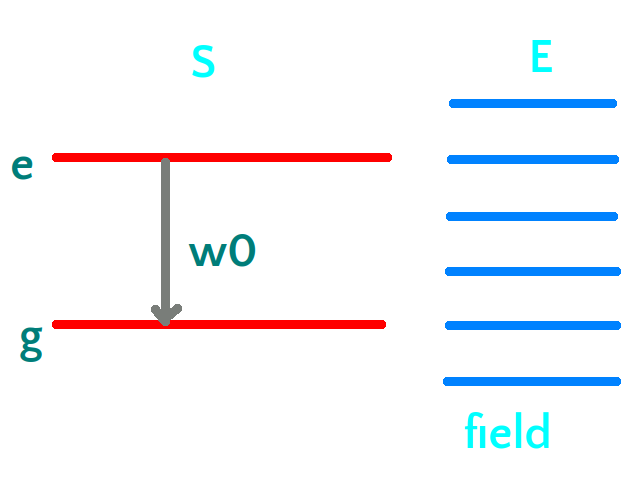
\includegraphics[width=0.55\textwidth]{sbm.png}
\caption{Representación pictórica del sistema de Spin Boson Model (en adelante SBM). Un átomo de 2 niveles $\ket{e}$ y $\ket{g}$, con una diferencia de energía entre ambos de $\hslash\omega_0$. Se acopla dicho átomo con un campo electromagnético que contiene muchos niveles de energía.}
\end{figure} 
\section{Desarrollo y suposiciones}
Como se dijo anteriormente, el hamiltoniano del sistema completo se compone del hamiltoniano del sistema, del ambiente (que sumados dan un elemento de \textit{Hamiltoniano libre o sin interacción} y un elemento de interacción:
\begin{equation}\label{eq4.1}H=H_S+H_E+H_{SE}=H_0+H_I\end{equation}
Para el sistema a evaluar el reservorio será un sistema termodinámico que al contacto con otro sistema mantiene su temperatura, lo que implica que $H_E$ maximiza la entropía de Von Neumann:
\begin{equation}\label{eq4.2}S(\rho_E)=-Tr(\rho_E log \rho_E)\end{equation}
Lo que implica que, análogamente al ensemble canónico en termodinámica clásica, la matriz densidad para el ambiente coincida con el ensemble canónico cuántico:
\begin{equation}\label{eq4.3}\rho_E=\frac{e^{-\beta H_E}}{Tr(e^{-\beta H_E})}\end{equation}.
Esta será la base de algunas de las suposiciones que se verán a continuación. A partir de la Ecuación de Von Neumann:
\begin{equation}\label{eq4.4}\dot{\rho}=\frac{1}{i\hslash}[H,\rho]\end{equation}
Si se empieza a ocupar el cuadro de interacción (a partir de \ref{eq4.4}), la matriz densidad queda:
\begin{equation}\label{eq4.5} \tilde{\rho}_{I}(t)=e^{\frac{iH_0t}{\hslash}}\rho(t)e^{-\frac{iH_0t}{\hslash}}\end{equation}
y su derivada en el tiempo por ende es
\begin{equation}\label{eq4.6} \dot{\tilde{\rho}}_{I}(t)=\frac{i}{\hslash}[H_0,\tilde{\rho}_{I}(t)]-\frac{i}{\hslash}[H_0,\tilde{\rho}_{I}(t)]-\frac{i}{\hslash}[\tilde{H}_I(t)_,\tilde{\rho}_{I}(t)]=\frac{1}{i\hslash}[\tilde{H}_I(t)_,\tilde{\rho}_{I}(t)]\end{equation}
Trazando el \ref{eq4.5} en el ambiente se obtiene $\rho_S$ en el cuadro de interacción:
\begin{equation}\label{eq4.7}\tilde{\rho}_S(t)=Tr_E(\tilde{\rho}_I(t))\end{equation}
Tal que la ecuación de \ref{eq4.6} para $\tilde{\rho}_S$ es
\begin{equation}\label{eq4.8}\dot{\tilde{\rho}}_S(t)=\frac{1}{i\hslash} Tr_E[\tilde{H}_I(t),\tilde{\rho}_I(t)]\end{equation} Al integrar \ref{eq4.6} resulta
\begin{equation}\label{eq4.9}\tilde{\rho}_I(t)=\frac{1}{i\hslash}[\tilde{H}_I(t),\tilde{\rho}_i(0)]+\frac{1}{i\hslash}\int_0^t dt_1[\tilde{H}_I(t),[\tilde{H}_I(t_1),\tilde{\rho_I}(t_1)]]\end{equation}
Y finalmente insertando \ref{eq4.9} en \ref{eq4.8}
\begin{equation}\label{eq4.10}\dot{\tilde{\rho}}_S(t)=\frac{1}{i\hslash}Tr_E[\tilde{H}_I(t),\tilde{\rho}_i(0)]+\frac{1}{i\hslash}\int_0^t dt_1Tr_E[\tilde{H}_I(t),[\tilde{H}_I(t_1),\tilde{\rho_I}(t_1)]]\end{equation}
El resultado obtenido en \ref{eq4.10} es un resultado exacto. Desde acá se empieza a construir la ecuación maestra microscópica a partir de las aproximaciones que se presentará.
\subsection{Aproximación de Born} Si la interacción entre el reservorio y el sistema es lo suficientemente débil entonces el estado del reservorio no es alterado. 
\begin{equation}\label{eq4.11}\tilde{\rho}_I(t)\simeq\tilde{\rho}_S(t)\otimes\rho_E\end{equation}
Siendo $\rho_E$ un estado termal como el mostrado en \ref{eq4.3}. Con lo anterior se puede sacar a $\rho_S$ de la traza de \ref{eq4.10} y separarlo de $\rho_E$ de la integral.
\begin{equation}\label{eq4.12}\dot{\tilde{\rho}}_S(t)=\frac{1}{i\hslash}Tr_E[\tilde{H}(t),\tilde{\rho}_s(0)\otimes\rho_E]+\frac{-1}{\hslash^2}\int_0^t dt_1 Tr_E[\tilde{H}_I(t),[\tilde{H}_I(t_1),\tilde{\rho_S}(t_1)\otimes\rho_E]]\end{equation}
\subsection{Acoplamiento Débil} 
El acoplamiento débil implica que el hamiltoniano de interación se puede descomponer en productos tensoriales de operadores $S_\alpha$ que solo opera en el sistema y $E_\alpha$ que solo operan en el ambiente:
\begin{equation}\label{eq4.13}H_i=\sum_\alpha S_\alpha\otimes E_\alpha\end{equation}
Lo que también se hace válido en el cuadro de interacción:
\begin{equation}\label{eq4.14}\tilde{H}_i(t)=e^{\frac{iH_0t}{\hslash}}H_Ie^{\frac{-iH_0t}{\hslash}}=\sum_\alpha \hat{S}_\alpha (t)\otimes \hat{E}_\alpha(t) \end{equation}
Insertando en el primer sumando de \ref{eq4.12} 
\begin{equation}\label{eq4.15}\frac{1}{i\hslash}Tr_E[\tilde{H}_I(t),\tilde{\rho}_I(0)]=\frac{1}{i\hslash}\sum_\alpha Tr_E ([\tilde{S}_\alpha(t)\otimes\tilde{E}_\alpha(t),\tilde{\rho}_S(0)\otimes\rho_E])\end{equation}
Al ser la traza cíclica:
\begin{equation}\label{eq4.16}=\frac{1}{i\hslash}
\sum_\alpha <\tilde{E}_\alpha(t)>[\tilde{S}_\alpha(t),\tilde{\rho}_S(0)]\end{equation}
¿Qué es $<\tilde{E}_\alpha$? Simplemente el promedio de $\tilde{E}_\alpha$ en la distribución termal declarada para $E$. Corresponde recordar que en muchas ocasiones ese promedio se anula. Como ejemplo en el sistema donde $H_I$ tiene la forma (consiste en el acoplamiento de un sistema de 2 niveles con uno de modos vibracionales):
\begin{equation}\label{eq4.17}H_I=\sigma_z\otimes\sum_k(g_kb_k+g_k^*b_k^\dag)\end{equation}
En dicho sistema $<\tilde{E}_\alpha(t)>$ es combinación lineal de los promedios $<b_k>$ y $<b_k^\dag>$, que se anulan para una distribución termal, por lo que se cumple lo anterior.
Si en el sistema $<\tilde{E}_\alpha(t)>\neq 0$, siempre se puede hacer una \textcolor{red}{Aproximación de Campo Medio}, que no es más que sumar valores constantes a los valores de energía de manera que $<\tilde{E}_\alpha(t)>$ se vuelve $0$.
\begin{equation}\label{eq4.18}\begin{aligned}H_S \textcolor{red}{\rightarrow} H_S+\sum_\alpha S_\alpha<E_\alpha>\\ \textcolor{red}{\Rightarrow} H_I\textcolor{red}{\rightarrow} \sum_\alpha S_\alpha\otimes(E_\alpha-<E_\alpha>)\end{aligned}\end{equation}
Dicho esto se puede decir sin perder generalidad que para un sistema general $<\tilde{E}_\alpha(t)>=0$ (porque de no serlo se puede hacer lo anterior), por lo que solo sobrevive el segundo sumando de \ref{eq4.12}
\begin{equation}\label{eq4.19}\dot{\tilde{\rho}}_S(t)=\frac{-1}{\hslash^2}\int_0^t dt_1 Tr_E[\tilde{H}_I(t),[\tilde{H}_I(t_1),\tilde{\rho_S}(t_1)\otimes\rho_E]]\end{equation}
Escribiendo $\tilde{H}_I$ en la descomposición sugerida en \ref{eq4.14}
\begin{equation}\label{eq4.20}\begin{aligned} Tr_E[\tilde{H}_I(t),[\tilde{H}_I(t_1),\tilde{\rho}_I(t_1)]]=\sum_{\alpha\beta} Tr_E(\tilde{E}_\alpha^\dag (t)\tilde{E}_\beta(t_1)\rho_E)[\tilde{S}_\beta(t_1)\tilde{\rho}_S(t_1)\tilde{S}_\alpha^\dag(t)\\ -\tilde{S}_\alpha^\dag(t)\tilde{S}_\beta(t_1)\tilde{\rho}_S(t_1)]+h.c.\end{aligned}\end{equation}
Lo anterior aprovechó también que la traza es cíclica. Dado que se observan trazas productos entre funciones componentes de $H_I$ a distintos tiempos ($t$ y $t_1$), corresponde evaluar la \textcolor{red}{Función de Correlación}.
\begin{equation}\label{eq4.21}G_{\alpha\beta}(t,t_1)=<\tilde{E}_\alpha^\dag (t)\tilde{E}_\beta(t_1)>=Tr_E(\tilde{E}_\alpha^\dag (t)\tilde{E}_\beta(t_1)\rho_E)\end{equation}
Con lo que \ref{eq4.20} queda:
\begin{equation}\label{eq4.22}\begin{aligned} Tr_E[\tilde{H}_I(t),[\tilde{H}_I(t_1),\tilde{\rho}_I(t_1)]]=\sum_{\alpha\beta}     G_{\alpha\beta}(t,t_1)[\tilde{S}_\beta(t_1)\tilde{\rho}_S(t_1)\tilde{S}_\alpha^\dag(t)\\ -\tilde{S}_\alpha^\dag(t)\tilde{S}_\beta(t_1)\tilde{\rho}_S(t_1)]+h.c.\end{aligned}\end{equation}
\subsection{Primera Aproximación de Markov}
También llamada aproximación \textcolor{red}{time-local} o \textcolor{red}{tiempo local}. Resulta de considerar una propiedad interesante de la función de correlación. Al descomponer la definición de \ref{eq4.21} con la definición de cuadro de interacción
\begin{equation}\label{eq4.23}G_{\alpha\beta}(t,t_1)=Tr_E((e^{\frac{iH_0t}{\hbar}}E_\alpha^\dag e^{-\frac{iH_0t}{\hbar}})(e^{\frac{iH_0t_1}{\hbar}}E_\beta e^{-\frac{iH_0t_1}{\hbar}})\rho_E)\end{equation}
Haciendo una transformación cíclica en \ref{eq4.23}
\begin{equation}\label{eq4.24}G_{\alpha\beta}(t,t_1)=Tr_E((e^{\frac{iH_0(t-t_1)}{\hbar}}E_\alpha^\dag e^{-\frac{iH_0(t-t_1}{\hbar}})E_\beta\rho_E)\end{equation}
Entonces, si se nombre $\tau=t-t_1$, finalmente se demuestra que la función de correlación no depende de los 2 tiempos como 2 variables separadas sino de una sola: de la distancia entre ambos tiempos.
\begin{equation}\label{eq4.25}G_{\alpha\beta}(t,t_1)=G_{\alpha\beta}(\tau,0)\end{equation}
Por lo tanto, formalmente la primera aproximación de Markov consiste en asumir que la función de correlación depende del tiempo $\tau=t-t_1$. Esto es lo que también se llama \textcolor{red}{localidad del tiempo}. La justificación de esto tiene que ver con el llamado \textcolor{red}{Tiempo de Correlación} $t_c$, que es el tiempo en el cual las correlaciones del reservorio son relevantes. Al mirar la dinámica en la escala de tiempo se debe cumplir:
\begin{equation}\label{eq4.26}t>>t_C\textcolor{red}{\Rightarrow}\tilde{\rho}_S(t_1)\simeq\tilde{\rho_S}(t) \end{equation} Lo que implica que $\tau$ es del orden de $t_C$, o sea, que estamos en el pequeño intervalo de tiempo en que las correlaciones entre espacio y tiempo importan.\\
Si no se agrega esta aproximación, el resultado de la ecuación derivada de la Von Neumann incluirá convoluciones. Por tanto, la aproximación es útil para tener una ecuación maestra manejable.
\subsection{Aproximación Secular}
Para introducir esta aproximación, se comenzará introduciendo la \textcolor{red}{Descomposición Espectral} de un operador. Para un hamiltoniano $H_S$ no degenerado con sus autoestados rotulados como $\ket{a}$ o $\ket{b}$ la descomposición espectral de un operador $S_\alpha$ es
\begin{equation}\label{eq4.27}S_\alpha(\omega)=\sum_{a,b}\delta(\omega_{a,b}-\omega)\ket{a}\bra{a}S_\alpha\ket{b}\bra{b}\end{equation}
Siendo $\frac{E_b-E_a}{\hbar}$, lo que hace la descomposición finalmente es permitir la escritura del operador como una función de frecuencias resonante con los elementos de matriz:
\begin{equation}\label{eq4.28}\sum_\omega S_\alpha(\omega)=\sum_\omega\sum_{a,b}\delta(\omega_{a,b}-\omega)\ket{a}\bra{a}S_\alpha\ket{b}\bra{b}=S_\alpha\end{equation}
Como ejemplo, se observa la descomposición espectral del operador $\sigma_z$
\begin{equation}\label{eq4.29}\sigma_z(\omega)=\delta(\omega)\ket{0}\bra{0}-\delta(\omega)\ket{1}\bra{1}\end{equation}
Tal que sumado sobre $\omega$ se obtiene finalmente $\sigma_z$.
Esto se aprovecha para descomponer un operador en cuadro de interacción:
\begin{equation}\label{eq4.30}\tilde{S}_\beta(t_1)=e^{\frac{iH_s t_1}{\hbar}}S_\beta e^{-\frac{iH_s t_1}{\hbar}}=\sum_\omega\sum_{a,b}\delta(\omega_{a,b}-\omega)e^{\frac{iH_s t_1}{\hbar}}\ket{a}\bra{a}S_\beta\ket{b}\bra{b}e^{-\frac{iH_s t_1}{\hbar}}\end{equation}
Aplicando el Hamiltoniano en dónde está 
\begin{equation}\label{eq4.31}e^{\frac{iH_s t_1}{\hbar}}\ket{a}=e^{i\omega_a t_1}\ket{a},\bra{b}e^{-\frac{iH_s t_1}{\hbar}}=\bra{b}e^{-i\omega_b t_1}\end{equation}
Al reemplazar en \ref{eq4.30}
\begin{equation}\label{eq4.32}\tilde{S}_\beta(t_1)=\sum_\omega\sum_{a,b}\delta(\omega_{a,b}-\omega)e^{\frac{-i\omega_{ab}t_1}{\hslash}}\ket{a}\bra{a}S_\beta\ket{b}\bra{b}=\sum_\omega e^{-i\omega t}S_\beta(\omega)\end{equation}
Y conjugando \ref{eq4.32} se obtiene la descomposición para el operador conjugado:
\begin{equation}\label{eq4.33}\tilde{S}_\alpha^\dag (t)=\sum_{\omega^\prime}e^{i\omega^\prime t}S_\alpha^\dag(\omega^\prime)\end{equation}
Al reescribir \ref{eq4.19} usando \ref{eq4.22}, \ref{eq4.32} y \ref{eq4.33} resulta
\begin{equation}\label{eq4.34}\dot{\tilde{\rho}}_S(t)=\sum_{\alpha\beta}\sum_{\omega\omega^\prime}\int_0^t dt_1 G_{\alpha\beta}(t,t_1)e^{-i(\omega t_1+\omega^\prime t)}(S_\beta(\omega)\tilde{\rho}_SS_\alpha^\dag(\omega^\prime)-S_\alpha^\dag(\omega^\prime)S_\beta(\omega)\tilde{\rho}_S)+h.c.\end{equation}
Redefiniendo la integral que aparece en \ref{eq4.34}
\begin{equation}\label{eq4.35}\Gamma_{\alpha\beta}(\omega,t)=\int_0^t G_{\alpha\beta}(\tau)e^{i\omega\tau} d\tau \end{equation}
Se reescribe \ref{eq4.34}
\begin{equation}\label{eq4.36}\dot{\tilde{\rho}}_S(t)=\sum_{\alpha\beta}\sum_{\omega\omega^\prime}\Gamma_{\alpha\beta}(\omega,t)e^{i(\omega^\prime-\omega)t}(S_\beta(\omega)\tilde{\rho}_SS_\alpha^\dag(\omega^\prime)-S_\alpha^\dag(\omega^\prime)S_\beta(\omega)\tilde{\rho}_S)+h.c.\end{equation}
Y surge la llamada \textcolor{red}{Ecuación Maestra Tiempo Local sin aproximación secular}.\\

La aproximación secular consiste en asumir que el término exponencial $e^{i(\omega^\gamma-\omega)t}$ tiene como máximo valor $1$ (cuando $\omega=\omega^\prime$) y se puede simplificar asumiendo que 
cuando $\omega\neq\omega^\prime$ existe una escala de tiempo del orden de $\lvert\omega^\prime-\omega\rvert^{-1}$, con frecuencias del órden del $GHz$
\begin{equation}\label{4.37}\tau>>\lvert\omega^\prime-\omega\rvert^{-1}\textcolor{red}{\Rightarrow} e^{i(\omega^\prime-\omega)t}\delta(\omega^\prime-\omega)\end{equation} Con lo que \ref{eq4.36} se reescribe \begin{equation}\label{eq4.38}\dot{\tilde{\rho}}_S(t)=\sum_{\alpha\beta}\sum_{\omega}\Gamma_{\alpha\beta}(\omega,t)(S_\beta(\omega)\tilde{\rho}_SS_\alpha^\dag(\omega)-S_\alpha^\dag(\omega)S_\beta(\omega)\tilde{\rho}_S)+h.c.\end{equation}
Siendo esta la \textcolor{red}{Ecuación Maestra Tiempo Local con aproximación secular}.
Se puede reescribir la función $\Gamma_{\alpha\beta}(\omega,t)$ en función de otro operador $\gamma_{\alpha\beta}(\omega,t)$.
\begin{equation}\label{eq4.39}\gamma_{\alpha\beta}(\omega,t)=\sum_{\alpha\beta\gamma}(\Gamma_{\alpha\beta}(\omega,t)+\Gamma^*_{\alpha\beta}(\omega,t))\end{equation}
Análogamente se puede definir la función $\lambda_{\alpha\beta}(\omega,t)$
\begin{equation}\label{eq4.40}\lambda_{\alpha\beta}(\omega,t)=\frac{1}{2i}\sum_{\alpha\beta\gamma}(\Gamma_{\alpha\beta}(\omega,t)-\Gamma^*_{\alpha\beta}(\omega,t))\end{equation}
Reescribiendo \ref{eq4.38}, ahora con el hermítico conjugado debidamente escrito: 
\begin{equation}\label{eq4.41}\begin{aligned}\dot{\tilde{\rho}}_S(t)=\sum_{\alpha\beta}\sum_{\omega}\Gamma_{\alpha\beta}(\omega,t)(S_\beta(\omega)\tilde{\rho}_SS_\alpha^\dag(\omega)-S_\alpha^\dag(\omega)S_\beta(\omega)\tilde{\rho}_S)\\ +\sum_{\alpha\beta}\sum_{\omega}\Gamma^*_{\beta\alpha}(\omega,t)(S_\beta(\omega)\tilde{\rho}_SS_\alpha^\dag(\omega)-\tilde{\rho}_SS_\alpha^\dag(\omega)S_\beta(\omega))\end{aligned}\end{equation}
Reemplazando \ref{eq4.39} y \ref{eq4.40} en \ref{eq4.41}
\begin{equation}\label{eq4.42}\begin{aligned}\dot{\tilde{\rho}}_S(t)=\sum_{\alpha\beta\omega}\frac{\gamma_{\alpha\beta}(\omega,t)}{2}(2S_\beta(\omega)\tilde{\rho}_S(t)S_\alpha^\dag(\omega)-\{S_\alpha^\dag(\omega)S_\beta(\omega),\tilde{\rho}_S(t)\})\\ -i\sum_{\alpha\beta\omega}\lambda_{\alpha\beta}(\omega,t)[S_\alpha^\dag(\omega)S_\beta(\omega),\tilde{\rho}_S(t)]\end{aligned}\end{equation}
Lo que que es otra forma de escribir la \textcolor{red}{Ecuación Maestra, Tiempo Local y Secular}
Definiendo el elemento de \textcolor{red}{Lamb Shift} del Hamiltoniano:
\begin{equation}\label{eq4.43}H_{LS}(t)=\sum_{\alpha\beta\omega}\lambda_{\alpha\beta}(\omega,t)S_\alpha^\dag(\omega)S_\beta(\omega)\end{equation}
De manera que \ref{eq4.42} finalmente queda:
\begin{equation}\label{eq4.44}\dot{\tilde{\rho}}_S(t)=-i[H_{LS}(t),\tilde{\rho}_i]+\sum_{\alpha\beta\omega}\frac{\gamma_{\alpha\beta}(\omega,t)}{2}(2S_\beta(\omega)\tilde{\rho}_S(t)S_\alpha^\dag(\omega)-\{S_\alpha^\dag(\omega)S_\beta(\omega),\tilde{\rho}_S(t)\})\end{equation}
\subsection{Segunda Aproximación de Markov}
La segunda aproximación de Markov hace suponer que las tasas $\Gamma(\omega,t)$ en realidad no dependen del tiempo, porque se usan como una integral impropia:
\begin{equation}\label{eq4.45}\int_0^t e^{i\omega\tau}G_{\alpha\beta}(\tau)d\tau\simeq\int_0^\infty e^{i\omega\tau}G_{\alpha\beta}(\tau)d\tau\end{equation}
Y entonces $\gamma_{\alpha\beta}(\omega)$ con la segunda aproximación de Markov es:
\begin{equation}\label{eq4.46}\gamma_{\alpha\beta}(\omega)=\int_0^\infty e^ {i\omega\tau}G_{\alpha\beta}(\tau)d\tau+\int_0^\infty e^ {-i\omega\tau}G^*_{\alpha\beta}(\tau)d\tau\end{equation}
Y usando la propiedad $G_{\alpha\beta}^*(\tau)=G_{\alpha\beta}(-\tau)$. además de cambiar de variable $\tau=-\tau$ en la segunda integral de \ref{eq4.46} \begin{equation}\label{eq4.47}\gamma_{\alpha\beta}(\omega)=\int_0^\infty e^ {i\omega\tau}G_{\alpha\beta}(\tau)d\tau+\int_{-\infty}^0 e^ {i\omega\tau}G_{\alpha\beta}(\tau)d\tau=\int_{-\infty}^\infty e^ {i\omega\tau}G_{\alpha\beta}(\tau)d\tau\end{equation}
Con lo que la \textcolor{red}{Ecuación Maestra Microscópica} finalmente queda:
\begin{equation}\label{eq4.48}\dot{\tilde{\rho}}_S(t)=-i[H_{LS}(t),\tilde{\rho}_i]+\sum_{\alpha\beta\omega}\gamma_{\alpha\beta}(\omega)(S_\beta(\omega)\tilde{\rho}_S(t)S_\alpha^\dag(\omega)-\frac{1}{2}\{S_\alpha^\dag(\omega)S_\beta(\omega),\tilde{\rho}_S(t)\})\end{equation}
Además, si se vuelve al cuadro de Schrodinger la ecuación maestra queda:
\begin{equation}\label{eq4.49}\dot{\tilde{\rho}}_S(t)=-i[H_{S}(t)+H_{LS}(t),\tilde{\rho}_i]+\sum_{\alpha\beta\omega}\gamma_{\alpha\beta}(\omega)(S_\beta(\omega)\tilde{\rho}_S(t)S_\alpha^\dag(\omega)-\frac{1}{2}\{S_\alpha^\dag(\omega)S_\beta(\omega),\tilde{\rho}_S(t)\})\end{equation}
Como comentario final, el Lamb Shift hace una contribución marginal al cálculo de elementos de matriz, excepto para el Laser.
\section{Ejemplos}
\subsection{Spin Boson Model}
Para mostrar la gran utilidad de la ecuación maestra microscópica se usará en SBM, donde el spin es el sistema y el ambiente está formado por bosones, que pueden ser fotones o fonones. Para todo el análisis $\hslash=1$\\

Su Hamiltoniano está compuesto por sumandos que representan al sistema, al ambiente, al \textit{pure dephasing} y a los intercambios de energía:
\begin{equation}\label{eq4.50}H=\frac{1}{2}\omega_0\sigma_z+\sum_k\omega_kb_k^\dag b_k+\frac{1}{2}\sigma_z\sum_k(g_kb_k+g_k^*b_k^\dag)+\frac{1}{2}\sigma_x\sum_k(\lambda_k b_k+\lambda_k^*b_k^\dag)\end{equation}
Como comentario para explicar el hamiltoniano anterior, el operador $\sigma_z$ solo añade fases, mientras el $\rho_x$ hace cambios de estado.\\ Los bosones cumplen como álgebra: \begin{equation}\label{eq4.51}[b_k,b_k^\dag]=\delta_{kk^\prime}\textcolor{red}{\Rightarrow} <b_k^\dag,b_{k^\prime}>=n(\omega_k)\delta_{kk^\prime}\end{equation}
 Si para cualquier $k$ $\lambda_k=0$, solo existe como elemento de interacción el de \textit{pure dephasing} y la descomposición en los operadores requeridos es simple.
 \begin{equation}\label{eq4.52}H_I=\frac{1}{2}\sigma_z\sum_k(g_kb_k+g_k^*b_k^\dag)\textcolor{red}{\Rightarrow} S_1=\frac{1}{2}\sigma_z, E_1=\sum_k(g_kb_k+g_k^*b_k^\dag) \end{equation}
 Poniendo estos operadores en \ref{eq4.49} (despreciando el Lamb Shift).
 \begin{equation}\label{eq4.53}\dot{\tilde{\rho}}(t)=-i[H_S(t),\tilde{\rho}_i]+\gamma_{11}(\omega)(S_1(\omega)\tilde{\rho}_S(t)S_1^\dag(\omega)-\frac{1}{2}\{S_1^\dag(\omega)S_1(\omega),\tilde{\rho}_S(t)\})\end{equation} 
Colocando la definición de $S_1$ de \ref{eq4.52},\ref{eq4.53}, (usando que $\sigma_z\sigma_z=\mathbb{I}$ queda:
 \begin{equation}\label{eq4.54}\dot{\tilde{\rho}}(t)=-i[H_S(t),\tilde{\rho}_i]+\frac{\gamma_{11}(\omega)}{4}(\sigma_z\tilde{\rho}_S\sigma_z-\tilde{\rho}_S)\end{equation} 
 Para completar la ecuación de este sistema, corresponde hallar $\gamma_{11}(\omega)$ usando las reglas exhibidas al derivar la ecuación maestra microscópica:
 \begin{equation}\label{eq4.55}\gamma_{11}(0,t)=\Gamma_{11}(0,t)+(\Gamma_{11}(0,t))^*=2Re\{\int_0^t G_{11}(\tau)e^{i\omega_k \tau}\}=2Re\{\int_0^t <\tilde{E}_1(\tau)E_1(0)>d\tau\}\end{equation}
A partir de la definición de $E_1$ en \ref{eq4.52} se escribe ese operador en marco de interacción:
\begin{equation}\label{eq4.56}\tilde{E}_1(\tau)=\sum_k(g_kb_ke^{-i\omega_k\tau}+g_k^*b_k^\dag e^{i\omega_k\tau})\end{equation}
Con \ref{eq4.56} se puede escribir la correlación requerida en la integral de \ref{eq4.55} \begin{equation}\label{eq4.57}<\tilde{E}_1(\tau)E_1(0)>=\sum_{kk^\prime}(g_kg_k^*<b_kb_k^\dag>e^{-i\omega_k\tau}+g_k^*g_k<b_k^\dag b_k> e^{i\omega_k\tau})\end{equation}
Y usando la estadística de \ref{eq4.51}, se obtiene de \ref{eq4.57}
 \begin{equation}\label{eq4.58}<\tilde{E}_1(\tau)E_1(0)>=\sum_{kk^\prime}\lvert g_k\rvert^2((1+n(\omega_k))e^{-i\omega_k\tau}+n(\omega_k) e^{i\omega_k\tau})\end{equation}
 Y reemplazando en \ref{eq4.55}
 \begin{equation}\label{eq4.59}\gamma_{11}(0,t)=2Re\{\int_0^t \sum_{kk^\prime}\lvert g_k\rvert^2((1+n(\omega_k))e^{-i\omega_k\tau}+n(\omega_k) e^{i\omega_k\tau}) d\tau\}\end{equation}
 Como la parte real de la exponencial compleja es un coseno:
  \begin{equation}\label{eq4.60}\gamma_{11}(0,t)=2 \int_0^t \sum_{kk^\prime}\lvert g_k\rvert^2((1+n(\omega_k))cos(\omega_k\tau)+n(\omega_k) cos(i\omega_k\tau)) d\tau\end{equation}
  E integrando los cosenos:
\begin{equation}\label{eq4.61}\gamma_{11}(0,t)=2\sum_{kk^\prime}\lvert g_k\rvert^2(1+n(\omega_k))+n(\omega_k))\frac{sin(\omega_k t)}{\omega_k} d\tau\end{equation}
Pasando \ref{eq4.61} al continuo:
\begin{equation}\label{eq4.62}\gamma_{11}(\omega,t)=2\int_0^\infty D(\omega)\lvert g(\omega)\rvert^2(1+2n(\omega_k))\frac{sin(\omega)}{\omega} d\omega\end{equation}
$n(\omega_k)$, usando el gran canónico cuántico:
\begin{equation}\label{eq4.63}2n(\omega)+1=\frac{e^{\frac{\beta\hslash\omega}{2}}+e^{-\frac{\beta\hslash\omega}{2}}}{e^{\frac{\beta\hslash\omega}{2}}-e^{-\frac{\beta\hslash\omega}{2}}}=cotanh(\frac{\beta\hslash\omega}{2})\end{equation}
Con lo que finalmente:
\begin{equation}\label{eq4.64}\gamma_{11}(\omega,t)=2\int_0^\infty D(\omega)\lvert g(\omega)\rvert^2cotanh(\frac{\beta\hslash\omega}{2})\frac{sin(\omega)}{\omega} d\omega=2\gamma(t)\end{equation}
Tal que la ecuación maestra finalmente queda:
\begin{equation}\label{eq4.65}\dot{\rho}_S=-i[H_S,\rho_S]+\frac{\gamma(t)}{2}(\gamma_Z\rho_S\gamma_Z-\rho_S)\end{equation}
Por lo que se muestra que el sistema, solo con \textit{pure dephasing} define un $\gamma$ \textcolor{red}{dependiente de la temperatura}, que a su vez define mucha física.\\

Concluyendo el análisis para SBM, se puede decir que los primeros elementos del integrando de \ref{eq4.64} se le puede definir como \textcolor{red}{Función de Densidad Espectral}
\begin{equation}\label{eq4.66}J(\omega)=\lvert g(\omega)\rvert^2 D(\omega)\end{equation}
En la mayoría de los casos $J(\omega)$ tiene forma $\sim \omega^S e^{-\frac{\omega}{\omega_C}}$, siendo $\alpha$ el acoplamiento, $S$ la dimensionalidad del sistema y $\omega_C$ la llamada \textcolor{red}{Frecuencia de Corte}. \\

En fonones de baja frecuencia se puede decir que:
\begin{equation}\label{eq4.67}\lvert g(\omega)\rvert^2\simeq\omega. D(\omega)\simeq \omega^{d-1} \textcolor{red}{\Rightarrow} J(\omega)\simeq\omega^d \end{equation}
El sistema fonónico se puede clasificar a partir del valor de $S$, Si $S=1$, el sistema es \textcolor{red}{óhmico}. Si es menor, es \textcolor{red}{subpoissoniano} y si es mayor es \textcolor{red}{superpoissoniano}. Esto último es la demostración de que a partir de elementos de la ecuación maestra se puede derivar \textcolor{red}{Mucha Física}.
\begin{thebibliography}{XXX0000}
  \bibitem{Omar} Jimenez, 0. Apunte Información Cuántica 1
    \bibitem{Method} Luo S, Quantum discord for two-qubit systems. Phys. Rev. A 77, 042303 (2008)
  \bibitem{Method2} Gallego M., Orszag M. Death and revival of the quantum discord and the
measurement-induced disturbance. J. Opt. Soc. Am. B Vol. 29, No. 7 (2012)
\bibitem{Ali} Ali M., Rau A.R.P. , Alber G. Quantum Discord for two-qubit X states. Phys. Rev. A 81, 042105 (2010)
  \bibitem{Results} Gallego M., Coto R., Orszag M. Generation of quantum correlations for
two qubits through a common reservoir. Phys. Scr. T147 (2012) 014012 (4pp)
\end{thebibliography}
\chapter{Quantum Jumps}
Aparte de la ecuación maestra, existe otro tipo de métodos. Si se sigue insistiendo en usar la Ecuación de Schrodinger para un sistema abierto, se debe agregar elementos estocásticos a la dinámica. De ahí surgen los llamados \textcolor{red}{Quantum Jumps}, que se pueden entender como la manera cuántica de explicar las fluctuaciones, debido que hacer la Ecuación de Schrodinger estocástico implica agregar Ruido. \\

Por lo general el ruido se estudia en el cuadro de Heisenberg, pero que quiere evitar para tener cálculos más simples. En el siguiente análisis, más que ruido se analizará la pérdida de excitaciones. Los sistemas markovianos ya tienen una teoría de Quantum Jumps ya desarrollada, mientras que para sistemas no markovianos el uso de Quantum Jumps es relativamente reciente. 
\section{Quantum Jumps Markovianos}
El siguiente desarrollo está basado en el hecho en  \cite{Carmichael} y \cite{Orszag2}. Se un estado inicial sin ruido y puro. Si la ecuación de Schrodinger tiene $N$ variables mientras las ecuaciones de maestras tienen $N^2$ variables.El método consiste en agregar al Hamiloniano libre del sistema un conjunto de operadores.
\begin{equation}\label{eq5.1}H=H_S-\frac{i\hslash}{2}\sum_m C_m^\dag C_m\end{equation}
Cuando  $C_m$ los llamados \textcolor{red}{Canales de Disipación}. Como un ejemplo aparecen las pérdidas atómicas o fotónicas:
\begin{equation}\label{eq5.2}C_m^{atom}=\sqrt{\gamma}\sigma^-, C_m^{photon}=\sqrt{\kappa}a\end{equation} De manera que el Hamiltoniano puede ser:
\begin{equation}\label{eq5.3}H=\frac{\hslash\omega}{2}\sigma_Z-\frac{i\hslash}{2}\gamma\sigma^+\sigma^-=\hslash(\frac{\omega}{2}-i\frac{\gamma}{2})\ket{e}\bra{e}-\frac{\hslash\omega}{2}\ket{g}\bra{g}\end{equation}
De manera que de la parte imaginaria del proyector imaginario del primer sumando del Hamiltoniano se puede derivar la inestabilidad del sistema.\\

Para que los Quantum Jumps funcionen la probabilidad de que se produzca un salto debe ser baja, lo que implica que la dinámica funciona como aproximación. 
\begin{equation}\label{eq5.4}\delta p_m(t_n)=\Delta t \bra{\phi(t_n)}C_m^\dag C_m\ket{\phi(t_n)}\end{equation}
siendo el intervalo de tiempo entre $0$ y $t_n$ dividido en $n$ intervalos infinitesimales $\Delta t$. Y el indicador de ocurrencia de salto sería:
\begin{equation}\label{eq5.5}\delta p(t_n)=\sum_m \delta p_m(t_n)\end{equation}
Se genera entonces un número aleatorio $r_n$ uniformente distribuido entre 0 y 1 tal que si $r_n\geq\delta p(t_n)$ no se produce el salto y de caso contrario, si se produce.\\
\subsection{Evolución Temporal sin salto}
Algo que se ha omitido es que el estado debe permanecer normalizado, algo que cumple la evolución de un Hamiltoniano normal, pero no uno como el de \ref{eq5.1}, que \textcolor{red}{ya no es un operador hermítico}, y por lo tanto los autoestados evolucionados no necesariamente sean unitarios. Por lo tanto, corresponde hacer una \textcolor{red}{Normalización}. Si se escribe el estado luego de la evolución temporal:
\begin{equation}\label{eq5.6}\ket{\phi^B(t_{n+1})}=e^{-\frac{iH\Delta t}{\slash}}\ket{\phi^B(t_{n})}\end{equation}
Al hacer un producto interno entre estados
\begin{equation}\label{eq5.7}\bra{\phi^B(t_{n+1})}\ket{\phi^B(t_{n+1})}\neq\bra{\phi(0)}\ket{\phi(0)}\end{equation} Debido a la no hermiticidad. Como ejemplo, para un estado que evoluciona bajo \ref{eq5.3} para el estado inicial
\begin{equation}\label{eq5.8}\ket{\phi(0)}=c_g(0)\ket{g}+c_e(0)\ket{e}\end{equation}
Luego de la evolución temporal queda 
\begin{equation}\label{eq5.9}\ket{\phi^B(t)}=e^{\frac{i\omega t}{2}}c_g(0)\ket{g}+e^{\frac{-i\omega t}{2}}e^{\frac{-\gamma t}{2}}c_e(0)\ket{e}\end{equation}
Y el producto interno es:
\begin{equation}\label{eq5.10}\bra{\phi^B(t)}\ket{\phi^B(t)}=\lvert c_g(0)\rvert^2+\lvert c_e(0)e^{-\gamma t}\rvert^2 < 1\end{equation}
\subsection{Definición de salto cuántico}
En cambio, si la variable aleatoria indica que debe haber un salto, el estado evoluciona así:
\begin{equation}\label{eq5.11}\ket{\phi^S(t_{n+1})}=\frac{C_m\ket{\phi^S(t_n)}}{\sqrt{\bra{\phi^S(t_n)}C_m^\dag C_m\ket{\phi^S(t_n)}}}\end{equation}
A esto es a lo que se llama \textcolor{red}{salto cuántico}. Y quita una excitación al sistema. Es útil para representar fotodetectores. 
\subsection{Promediar sobre todas las trayectorias produce la ecuación maestra}
Con la siguiente derivación se demostrará que los métodos de Quantum Jumps y Ecuación Maestra son equivalentes, llegando al mismo resultado. Se empieza con un ciclo evolución-salto-evolución
\begin{equation}\label{eq5.12}\ket{\phi^S(t)}=e^{-\frac{iH(t-t^\prime)}{\hslash}}C_m\ket{\phi^B(t^\prime)}=e^{-\frac{iH(t-t^\prime)}{\hslash}}C_me^{\frac{-iHt^\prime}{\hslash}}\ket{\phi(0)}\end{equation}
Usando el ejemplo de \ref{eq5.3}, \ref{eq5.12} es
\begin{equation}\label{eq5.13}\ket{\phi^S(t)}=e^{-\frac{iH(t-t^\prime)}{\hslash}}\sqrt{\gamma}c_e(0)e^{\frac{-iHt^\prime}{\hslash}}\ket{g}=c_e(0)\sqrt{\gamma}e^{\frac{i\omega}{2}(t-2t^\prime}e^{\frac{-\gamma t^{\prime}}{2}}\ket{g}\end{equation}
Desde \ref{eq5.12} se puede llegar a la ecuación maestra de distintas formas. En lo que resta de sección, siguiendo \cite{Orszag2}, se usará un tiempo discretizado.
\begin{equation}\label{eq5.14}\bar{\rho}_c(t_{n+1})=\ket{\bar{\phi}(t_{n+1})}\bra{\bar{\phi}(t_{n+1})}\end{equation}
Si se considera que en el intervalo entre $t_n$ y $t_{n+1}$ se produce una evolución temporal y no un salto:
\begin{equation}\label{eq5.15}\bar{\rho}_c(t_{n+1})=e^{-\frac{i}{\hslash}H\Delta t}\ket{\bar{\phi}(t_n)}\bra{\bar{\phi}(t_n)}e^{\frac{i}{\hslash}H\Delta t}\end{equation}
Al ser $\Delta t$ un intervalo pequeño, las exponenciales de \ref{eq5.14} se pueden aproximar en Taylor:
\begin{equation}\label{eq5.16}\bar{\rho}_c(t_{n+1})=e^{-\frac{i}{\hslash}H\Delta t}\bar{\rho}_c(t_n)e^{\frac{i}{\hslash}H\Delta t}\simeq (\mathbb{I}-\frac{i}{\hslash}H\Delta t)\bar{\rho}_c(t_n)(\mathbb{I}+\frac{i}{\hslash}H\Delta t)\end{equation}
Lo que, considerando solo los elementos de primer orden es
\begin{equation}\label{eq5.17}\bar{\rho}_c(t_{n+1})\simeq \bar{\rho}_c(t_n)-\frac{i}{\hslash}[H,\bar{\rho}_c(t_n)]\Delta t\end{equation}
y usando la definición de H de \ref{eq5.17} queda
\begin{equation}\label{eq5.18}\dot{\bar{\rho}}_c(t_n) \simeq\frac{\bar{\rho}_c(t_{n+1})-\bar{\rho}_c(t_n)}{\Delta t}=\frac{-i}{\hslash}[H_s,\rho_c(t_n)]-\frac{1}{2}\{\sum_m C_m^\dag C_m,\bar{\rho}_c(t_n)\}\end{equation}
Con lo que se obtiene la ecuación maestra pedida. Un comentario interesante es que hace falta un sumando tipo $C_m\bar{\rho}_c(t_n)C_m^\dag$ pero eso no es un problema ya que ese elemento sale luego de un quantum jump, los que son menos probables que las evoluciones temporales.\\

Otra forma de nombrar al método presentado de Quantum Jumps es como \textcolor{red}{Método de Montecarlo} (así se le llama por ejemplo en códigos como Qutip), dado que la forma en que se describe el método se puede clasificar como un ejemplo de dicho método de clasificación. El método de Quantum Jumps es muy útil para hallar valores de expectación, útiles experimentalmente.
\section{Derivación de Carmichael de Quantum Jumps}
El siguiente método para describir los Quantum Jumps (que a su vez está basado en \cite{Carmichael}, a diferencia del anterior, \textcolor{red}{No discretiza el tiempo}
Suponiendo que se puede encontrar un operador evolución temporal para el estado tal que cumpla:
\begin{equation}\label{eq5.19}\dot{\rho}=\mathcal{L}[\rho(t)]\textcolor{red}{\Rightarrow}\rho(t)=e^{-\mathcal{L}(t)\rho(0)}\end{equation}
Se puede separar dicho operador en 2, el \textcolor{red}{operador de dinámica sin saltos} y el \textcolor{red}{operador de salto}.
\begin{equation}\label{eq5.20}\mathcal{L}_B=\frac{-i}{\hslash}[H_S,\rho]-\frac{1}{2}\{\sum_m C_m^\dag C_m,\rho\}\end{equation}
\begin{equation}\label{eq5.21}\mathcal{L}_S=\sum_m C_m\rho C_m^\dag \textcolor{red}{\Rightarrow} \mathcal{L}=\mathcal{L}_B+\mathcal{L}_S\end{equation}
Como es sabido de la parte anterior, al calcular la variación del estado en el tiempo, existe una probabilidad de que exista evolución temporal y de que se produzca un salto. En este formalismo las probabilidades son:
\begin{equation}\label{eq5.22}p_b=\bra{\bar{\phi}^b(t)}\ket{\bar{\phi}^b(t)}, p_s=\bra{\bar{\phi}^s(t)}\ket{\bar{\phi}^s(t)}\end{equation}
Por lo que, considerando estas probabilidades, el truncado exacto producto de integrar \ref{eq5.19} es
\begin{equation}\label{eq5.23}\rho(t)=p_b\ket{\bar{\phi}^b(t)}\bra{\bar{\phi}^b(t)}+p_s\ket{\bar{\phi}^s(t)}\bra{\bar{\phi}^s(t)}\end{equation}
Luego se debe definir los vectores  y el tope de fotones permitidos para poder describir el salto. 
\section{Ejemplo:Modelo de Jaynes-Cumming con pérdidas}
El modelo de Jaynes Cumming tiene como Hamiltoniano Libre (considerando ${\hslash=1}$:
\begin{equation}{H_{JC}=\omega_a \sigma_+\sigma_-+\omega_c a^\dag a +g(a^\dag\sigma^-+a\sigma^+)}\end{equation} 
Para todo el desarrollo que viene $ {\omega_a=1}$,$ {\omega_c=1}$, $ {g=\frac{1}{1000}}$, por lo que el Hamiltoniano queda: 
\begin{equation}{H_{JC}=\sigma_+\sigma_-+a^\dag a +\frac{1}{1000}(a^\dag\sigma^-+a\sigma^+)}\end{equation} 
Considerando las siguientes definiciones matriciales:
\begin{equation}\begin{aligned}{\sigma^+=\ket{0}_A\bra{1}\otimes\mathbb{I}=\begin{pmatrix} 0&0&1&0 \\ 0&0&0&1 \\ 0&0&0&0 \\ 0&0&0&0 \end{pmatrix}}, {\sigma^-=\ket{1}_A\bra{0}\otimes\mathbb{I}=\begin{pmatrix} 0&0&0&0 \\ 0&0&0&0 \\ 1&0&0&0 \\ 0&1&0&0 \end{pmatrix}}\\ {a^\dag=\mathbb{I}\otimes\ket{0}_F\bra{1}=\begin{pmatrix} 0&1&0&0 \\ 0&0&0&0 \\ 0&0&0&1 \\ 0&0&0&0 \end{pmatrix}}, {a=\mathbb{I}\otimes\ket{1}_F\bra{0}=\begin{pmatrix} 0&0&0&0 \\ 1&0&0&0 \\ 0&0&0&0 \\ 0&0&1&0 \end{pmatrix}}\end{aligned}\end{equation}
Haciendo los productos, y sumando, el Hamiltoniano Jaynes-Cumming para un sistema de átomo de 2 niveles con campo de 1 modo es:
\begin{equation}{H_{JC}=\begin{pmatrix} 2.000 & 0.000 & 0.000 & 0.000 \\ 0.000 & 1.000 & 0.001 & 0.000 \\ 0.000 & 0.001 & 1.000 & 0.000 \\ 0.000 & 0.000 & 0.000  & 0.000\end{pmatrix}}\end{equation}
Los operadores de disipación, de acuerdo a la teoría, tienen la forma: 
\begin{equation}{S_1= \sqrt{2\Gamma}\sigma_-=\begin{pmatrix} 0&0&0&0& \\ 0&0&0&0 \\ \sqrt{2\Gamma}&0&0&0 \\ 0&\sqrt{2\Gamma} & 0&0 \end{pmatrix}, S_2=\sqrt{2\kappa}a=\begin{pmatrix} 0&0&0&0 \\ \sqrt{2\kappa}&0&0&0 \\ 0&0&0&0 \\ 0&0&\sqrt{2\kappa}&0\end{pmatrix} }\end{equation}
Si ${\kappa=0,1}$ y ${\Gamma=0,05}$, reemplazando queda:
\begin{equation}{S_1=\begin{pmatrix}0&0&0&0\\0&0&0&0\\ \sqrt{0,1}&0&0&0\\ 0&\sqrt{0,1}&0&0 \end{pmatrix},S_2=\begin{pmatrix}0&0&0&0 \\ \sqrt{0.2}&0&0&0 \\ 0&0&0&0 \\ 0&0&\sqrt{0.2}&0\end{pmatrix}}\end{equation}
Para poder programar la evolución en Quantum Jumps, es preciso seguir el siguiente algoritmo.
\begin{itemize}
\item\textcolor{ForestGreen}{\texttt{Definir operadores, Hamiltoniano Jaynes-Cumming y disipadores.}}
\item\textcolor{ForestGreen}{\texttt{Resolver ecuación maestra para 500 puntos y tiempo de 0 a 5.}}
\item\textcolor{ForestGreen}{\texttt{Definir 2 números aleatorios 500 veces.}}
\item\textcolor{ForestGreen}{\texttt{Usarlos para evaluar un si hay salto cuántico en el intervalo de 0 a 5.}}
\item\textcolor{ForestGreen}{\texttt{Repetir varias veces (cantidad variable de 100 a 600)}}
\item\textcolor{ForestGreen}{\texttt{Evaluar valores de expectación para g, e y número de partículas en gravedad promedio.}}
\item\textcolor{ForestGreen}{\texttt{Graficar los resultados para comparar ambos métodos.}}
\end{itemize}

Como se puede notar, el método de Quantum Jumps es un método fundamentalmente computacional, en el sentido que se puede entender como un algoritmo simple de implementar en un programa como Mathematica, MATLAB e incluso Python. Los resultados de aplicar Quantum Jumps tienden a converger a los resultados en ecuación maestra en alrededor de 500 a 1000 ejecuciones de dicho loop.
\begin{thebibliography}{XXX0000}
\bibitem{Carmichael} Carmichael An Open Systems Approach to Quantum Optics (1991)
\bibitem{Orszag2} Orszag, M. Quantum Optics, Third Edition (2013)
\end{thebibliography}
\chapter{Métodos de Espacio de Fases}
Otro método posible es analizar las evoluciones temporales del sistema (lo que comunmente se hace usando ecuaciones diferenciales maticiales) mediante métodos que permitan convertir estas ecuaciones en ecuaciones diferenciales algebraicas, más simples de resolver.
\section{Definición de Funciones de espacio de Fases}
Se comienza definiendo más precisamente cuáles son estas funciones y para qué sistemas físicos sirven. Todo este capítulo se ejemplificará buscando la función de Wigner para un estado termal.
\subsection{Función Q}
La función Q es la más fácil de definir matemáticamente, también es llamada \textcolor{red}{Distribución Antinormal}, y simplemente usa las componentes de la matriz densidad en estado coherente:
\begin{equation}\label{eq6.1}Q(\alpha, \alpha^*)=\frac{1}{\pi}\bra{\alpha}\rho\ket{\alpha}\end{equation}
\subsection{Función P}
La función P es llamada también \textcolor{red}{Distribución Normal}, y se puede construir implícitamente como los pesos de la integración en base coherente que lleva a la matriz densidad:
\begin{equation}\label{eq6.2}\rho=\int d^2 \alpha P
(\alpha,\alpha^*)\ket{\alpha}\bra{\alpha}\end{equation}
\subsection{Función de Wigner}
También conocida como \textcolor{red}{Distribución Simétrica} o \textcolor{red}{Transformación de Weyl}, es más complicada de definir aún, aunque puede hacerse en función de las posiciones y momentos. 
\begin{equation}\label{eq6.3}W(q_1...q_n;p_1...p_n)=(\frac{1}{\pi\hslash})^n \int_{-\infty}^\infty ... \int_{-\infty}^\infty dy_1...dy_n\psi^*\begin{pmatrix} q_1+y_1\\ ...\\ q_n+y_n\end{pmatrix}\psi\begin{pmatrix}q_1-y_1\\ ...\\ q_n-y_n\end{pmatrix}e^{\frac{2i}{\hslash}p_1q_1..p_nq_n}\end{equation}
La principal motivación para usar la función de Wigner es que es útil para representar las correcciones que le puede hacer la física cuántica a la Termodinámica. Como comentario es preciso recordar que la Función de Wigner \textcolor{red}{No se puede interpretar como probabilidad simultánea para posición y momentum}, aunque integrando en los $y_n$ se pueda ver como una especie de distribución de probabilidad.\\

Una propiedad interesante de la función de Wigner es que una matriz densidad $\rho$ no siempre puede ser totalmente representada por su respectiva función, ya que cuando se intentan interpretar los resultados de su distribución, donde debiesen aparecer probabilidades (que por definición son números positivos y que suman $1$ entre sí) aparecen números positivos y negativos.

\begin{equation}\label{eq6.4}\int dp W(q,p)=\bra{q}\rho\ket{q}=\lvert\psi(q)\rvert^2\end{equation}
\section{Uso de las funciones de espacio de fase}
¿Para qué se introducen estas funciones? Porque cumplen como propiedad que los valores de expectación cuánticos pueden expresarse en la misma forma que los promedios en Mecánica Estadísitica clásica. \begin{equation}\label{eq6.5} Tr(\hat{A},\hat{B})=\int\int dq dp A_\omega(q,p)B_\omega(q,p)\end{equation}
Si se asume que $\hat{B}=\rho$, se obtiene de \ref{eq6.5} la ecuación para valores de expectación:
 \begin{equation}\label{eq6.6} <\hat{A}>=\int\int dq dp W(q,p)A_\omega(q,p)\end{equation}
 Es probable que $W(q,p)$ no sea apropiado para representar algunas matrices densidad, pero de todas formas es útil para obtener los valores de expectación en varios casos.
 Otra utilidad del uso del método de espacio de fases es que se pueden obtener ecuaciones dinámicas a casos clásicos. Si se escribe \ref{eq6.3} para 1 dimensión:
 \begin{equation}\label{eq6.7}W(q;p)=\frac{1}{\pi\hslash} \int_{-\infty}^\infty dy \psi^*(q+y)\psi(qy)e^{\frac{2i}{\hslash}py}\end{equation}
 Se obtiene de la ecuación de Von Neumann para un $H$ estándar 
 \begin{equation}\label{eq6.8}H=\frac{p^2}{2m}+U(q)\textcolor{red}{\Rightarrow} \dot{W}(q,p,t)=\frac{-p}{m}\frac{\partial W(q,p,t)}{\partial q}+\frac{\partial W(q,p,t)}{\partial p}\end{equation}
\subsection{Funciones Características}
Se pueden definir también las llamadas \textcolor{red}{Funciones Características}, que no son otra cosa que las transformadas de Fourier de las funciones presentadas anteriormente. \\
Para una distribución \textcolor{red}{normal} u \textcolor{red}{ordenada}
\begin{equation}\label{eq6.9}X_N(\eta,\eta^*)=Tr(\rho e^{\eta a^\dag}e^{-\eta^* a})\end{equation}
Para una distribución \textcolor{red}{antinormal} o \textcolor{red}{antiordenada}
\begin{equation}\label{eq6.10}X_A(\eta,\eta^*)=Tr(\rho e^{-\eta^* a}e^{\eta a^\dag})\end{equation}
Para una distribución \textcolor{red}{simétrica}
\begin{equation}\label{eq6.11}X_W(\eta,\eta^*)=Tr(\rho e^{\eta a^\dag-\eta^* a})\end{equation}
Aunque ¿Sé significa más precisamente que un operador sea ordenado, antiordenado o simétrico? Tiene que ver con las posibles descomposiciones del operador en función de los operadores de subida y bajada. A continuación se muestran las descomposiciones ordenada, antiordenada y simétrica de un operador $\hat{A}$
\begin{equation}\label{eq6.12}\begin{aligned} \hat{A}_N=\sum_{n,m=0}^\infty c_{nm} (a^\dag)^n a^m \\ \hat{A}_N=\sum_{n,m=0}^\infty  c_{nm} a^m (a^{\dag})^n \\ \hat{A}_N=\sum_{n,m=0}^\infty  c_{nm} \{(a^\dag)^n a^m \}_{sym}\end{aligned}\end{equation}
Siendo en la tercera descomposición los elementos dependientes de $a$  y $a^\dag$ sumas simétricas de los posibles productos entre operadores. Para mejor comprensión, como ejemplo:
\begin{equation}\label{eq6.13}\{a^\dag a\}_{sym}=\frac{1}{2}(a^\dag a+aa^\dag)\end{equation}
De manera que insertando la descomposición simétrica de \ref{eq6.12} en \ref{eq6.6}
\begin{equation}\label{eq6.14}Tr(\rho\hat{A}_W)=\int d^2\alpha W(\alpha,\alpha^*)\sum_{n,m}^\infty C_{nm}\{\alpha^{*n}\alpha^m\}\end{equation}
\subsection{Transformación de Similaridad}
Si se descompone en la función $F$
\begin{equation}\label{eq6.15}F \textcolor{red}{\Rightarrow} F_\omega(\alpha.\alpha^*)=\frac{1}{\pi}\int d^2\eta e^{\eta^*\alpha-\eta\alpha^*}Tr(f(\alpha,\alpha^*)e^{\eta a^\dag-\eta^* a})=2Tr(D^\dag(\alpha)SD(\alpha)F(a,a^\dag))\end{equation}
En la segunda igualdad se usan las definiciones de \textcolor{red}{Operador Desplazamiento} y \textcolor{red}{Operador S}, lo que es darle a la función una descomposición similar a la del operador densidad. \begin{equation}\label{eq6.16}D(\alpha)=e^{\alpha a^\dag-\alpha^* a}. S=\frac{1}{2\pi}\int d^2\beta e^{\beta a^\dag-\beta^* a}\end{equation}
El operador S cumple las siguientes propiedades:
\begin{equation}\label{eq6.17}S=S^\dag=S^{-1}\end{equation}
\begin{equation}\label{eq6.18}S^{-1}a^\dag S=-a^\dag\end{equation}
\begin{equation}\label{eq6.19}S^{-1}aS=-a\end{equation}
Si se puede hacer una transformación en la descomposición 
\begin{equation}\label{eq6.20}F(a,a^\dag)\textcolor{red}{\Rightarrow}G(a,a^\dag)=V^{-1}F(a,a^\dag)V=F(\sigma a+\tau a^\dag,\mu a^\dag+\nu a)\end{equation}
Siendo $\tau$, $\sigma$, $\mu$ y $\nu$ son números complejos que cumple la propiedad $ \mu\sigma-\nu\tau=1$. La función $V$ no es necesariamente unitaria pero cumple la propiedad:
\begin{equation}\label{eq6.21}Im(\sigma^* \tau)\geq 0, Im(\nu\mu^*)\geq 0\end{equation}
Tal que luego de la transformación de $G$ es
\begin{equation}\label{eq6.22} G_\omega(\alpha.\alpha^*)=2Tr(D^\dag(\alpha)SD(\alpha)V^{-1}F(a,a^\dag)V)\end{equation}
Tal que la transformación cumple:
\begin{equation}\label{eq6.23}G_W(\alpha,\alpha^*)=F_W(\sigma \alpha+\tau \alpha^*,\mu \alpha^*+\nu \alpha)\end{equation}
Esto es llamado la \textcolor{red}{Transformación de Bogoliubov}, muy útil en superconductividad.
\section{Ejemplo: Condensado de Bose-Einstein}
Como ejemplo, se intentará aplicar métodos de espacio de fases para condensados de Bose-Einstein. El conteo de excitaciones es:
\begin{equation}\label{eq6.24}G(a,a^\dag,b,b^\dag)=e^{i(\mu a^\dag a +\nu b^\dag b)}\end{equation}
Para un estado termal, la matriz densidad es:
\begin{equation}\label{eq6.25}\rho=(1-e^{-\epsilon})^2 e^{-\epsilon(A^A +B^B)}\end{equation}
Para 1 modo $\epsilon=\beta\hslash\omega$ y las definiciones quedan:
\begin{equation}\label{eq6.26}\rho=\frac{e^{-\beta H_R}}{Z}=\frac{e^{-\beta H_R}}{Tr(e^{-\beta\hslash H_R})}=\frac{e^{-\beta\hslash H_R}}{e^{\beta\hslash\omega}-1}\end{equation}
Para \ref{eq6.26}, el Hamiltoniano es:
\begin{equation}\label{eq6.27}H_R=\sum_i \omega_i b_ib_i^\dag\end{equation}
La transformación de Bogoliubov que se puede aplicar es:
\begin{equation}\label{eq6.28}A=acosh\theta-b^\dag sin\theta, B=bcosh\theta-a^\dag sinh\theta\end{equation}
También se puede considerar $\alpha=cosh\theta$ u $\beta=sinh\theta$. Estos sistemas se observan, por ejemplo en las cavidades orgánicas. Para hallar el número de fotones por modo:
\begin{equation}\label{eq6.29}T(\mu.\nu.\epsilon)=Tr(\rho G(a,a^\dag,b,b^\dag))=\int\int d^2\alpha d^2 \beta W(\alpha,\alpha^*,\beta,\beta^*)G_W(\alpha,\alpha^*,\beta,\beta^*)\end{equation}
Y la función de Wigner para el estado termal es:
\begin{equation}\label{eq6.30}W^{(1)}=\frac{2}{\pi}tanh(\frac{\epsilon}{2})e^{-2\lvert\alpha\rvert^2 tanh(\frac{\epsilon}{2})}\end{equation}

\begin{thebibliography}{9}
\bibitem{Phase1} Englert, Fulling, Piloff, Optics Communications 208(1-3) - Published June 2002
\bibitem{Phase2} Frank, Rivera, Wolf, Phys. Rev. A 61, 054102 – Published 13 April 2000
\bibitem{Phase3} Deng, Hau, Yamamoto, Rev. Mod. Phys. 82, 1489 – Published 12 May 2010
\end{thebibliography}
\chapter{Ruido Cuántico}
Entendiendo como \textit{ruido} el resultado de fuerzas pequeñas y aleatorias, se puede considerar matemáticamente interesante analizar sus efectos en sistemas de variable continua. De aquí surge el \textcolor{red}{Cálculo Estocástico}.
Este texto funciona como una introducción de esta área aplicada a sistemas físicos simples. Esto con el objetivo de obtener métodos para evaluar sistemas cuánticos abiertos que aprovechan este formalismo.
\section{Ejemplos de Ruido}
\subsection{Movimiento Browniano}
Considerando como ejemplo el movimiento browniano. Este movimiento modela, por ejemplo, el comportamiento del Polen en el agua. Implica la existencia de \textcolor{red}{Fuerzas Aleatorias} que no necesariamente están en la misma dirección, con lo que se introduce el \textcolor{red}{Análisis de Langevin}.
\begin{equation}\label{eq7.1}(dx=u(t)dt): du=-\gamma u dt +\sqrt{f}dW(t)\end{equation} Donde $f$ es una constante y $dW(t)=\xi(t) dt$ inserta la variable aleatoria. El primer sumando corresponde a un elemento de decaimiento y el segundo incluye el ruido con el ingreso de aleatoreidad.
Esta ecuación diferencial tiene como solución.
\begin{equation}\label{eq7.2} u(t)=u(0)e^{-\gamma t}+\sqrt{f}\int_0^t ds e^{-\gamma(t-s)}\xi(s)\end{equation}
\subsection{Procesos Markovianos y Estadística}
Un proceso es \textcolor{red}{Markoviano} si no tiene memoria y $u(t)dt$ solo depende del $t$ anterior. Esto simplifica el análisis estadístico de \ref{eq7.1} usando como propiedad:
\begin{equation}\label{eq7.3}(dW(t)=\xi(t)dt) <\xi(t)>=0, <\xi(t)\xi(t^\prime)>=\delta(t-t^\prime) \end{equation}
Dicho análisis consiste en hallar su promedio y su varianza. En el promedio, por \ref{eq7.3}, solo influye el sumando determinístico
\begin{equation}\label{eq7.4}<u(t)>=u(0)e^{-\gamma t}\end{equation}
Mientras que la desviación estándar o varianza, se obtiene a partir de \ref{eq7.2} y la propiedad
\begin{equation}\label{eq7.5}(\Delta u(t))^2=<u(t)^2>-<u(t)>^2\end{equation}
resultando
\begin{equation}\label{eq7.6}(\Delta u(t))^2=f\int_0^t\int_0^{t^\prime}dt^\prime dt^{\prime\prime} e^{-\gamma(t-t^\prime)}e^{-\gamma(t-t^{\prime\prime})}<\xi(t^\prime)\xi(t^{\prime \prime})>\end{equation}
Y por \ref{eq7.3} el promedio de funciones aleatorias no es más que una delta, dejando solo una integral fácil de resolver.
\begin{equation}\label{eq7.7}(\Delta u(t))^2=f\int_0^t dt^\prime e^{-2\gamma(t-t^\prime)}=\frac{f}{2\gamma}(1-e^{-2\gamma t}) \end{equation}
También se puede evaluar el promedio del desplazamiento integrando lo obtenido en \ref{eq7.2}
\begin{equation}\label{eq7.8}<x(t)>=<\int_0^t ds u(s)>=\int_0^t ds <u(s)> =u(0)\int_0^t ds e^{-\gamma t}\end{equation}
Por lo que el resultado final de \ref{eq7.8} es:
\begin{equation}\label{eq7.9} (\Delta u(t))^2=\frac{u(0)}{\gamma}(1-e^{-\gamma t})\end{equation}
\subsection{Correlaciones y ruido}
Las funciones de correlación son muy ocupadas en Mecánica Cuántica. Un hecho importante a considerar es que 
\begin{equation}\label{eq7.10} <u(t_1)u(t_2)>\neq<u(t_1)><u(t_2)>\end{equation}
De manera análoga a cómo se obtiene varianzas, se puede decir que:
\begin{equation}\label{eq7.11}<u(t_1)u(t_2)>-<u(t_1)><u(t_2)>=\delta u(t_1)\delta u(t_2)\end{equation}
Lo que requiere incluir los sumandos aleatorios de las respectivas expresiones
\begin{equation}\label{eq7.12}\delta u(t_1)\delta u(t_2)=f\int_0^{t_1}\int_0^{t_2}ds_1 ds_2 e^{-\gamma(t_1-s_1)}e^{-\gamma(t_2-s_2)}<\xi(s_1)\xi(s_2)>\end{equation}
Haciendo el reemplazo de \ref{eq7.3} y considerando el tiempo menor (buscando la cota más baja para las correlaciones):
\begin{equation}\label{eq7.13}\delta u(t_1)\delta u(t_2)=f\int_{0}^{min(t_1,t_2)}ds_1 e^{-\gamma(t_1+t_2-2s_1)}=\frac{f}{2\gamma}(e^{\gamma\lvert t_1-t_2\rvert}-e^{-\gamma(t_1+t_2)})\end{equation}
Por lo que se puede concluir que \ref{eq7.10} es cierto y las correlaciones se vuelven no triviales precisamente por el ruido.
\subsection{Valores estacionarios para tiempos infinitos}
Si se calcula el desplazamiento integrando la velocidad
\begin{equation}\label{eq7.14}x(t)=\int_0^t ds u(0)e^{-\gamma s}+\sqrt{f}\int_0^t\int_0^s ds dt^\prime e^{-\gamma(s-t^\prime)} \xi(t^\prime)\end{equation}
Haciendo un cambio de variable para aíslar el término aleatorio \ref{eq7.14} se convierte en 
\begin{equation}\label{eq7.15}x(t)=\int_0^t ds u(0)e^{-\gamma s}+\sqrt{f}\int_0^t \int_{t^\prime}^t dt^\prime \xi(t^\prime) ds e^{-\gamma (s-t^\prime)}\end{equation}
Resolviendo la integral de s en \ref{eq7.15}\begin{equation}\label{eq7.16}x(t)=\int_0^t ds u(0)e^{-\gamma s}+\frac{\sqrt{f}}{\gamma}\int_0^t d t^\prime (1-e^{-\gamma(t-t^\prime)})\xi(t^\prime)\end{equation} Si se calcula la varianza para esta definición de x cuando t tiende a infinito se obtiene
\begin{equation}\label{eq7.17} (\Delta x(t))^2 \textcolor{red}{\Rightarrow} \frac{f}{\gamma^2}\end{equation}
\section{Ruido Clásico}
\subsection{Ruidos blancos y de color}
El ruido, como propiedad, tiene asociado un \textcolor{red}{espectro} de frecuencias, asociado con una función temporal mediante una Transformada de Fourier:
\begin{equation}\label{eq7.18}\tilde{x}(\omega+i\gamma, \tau)=\int_{-\infty}^{\infty} dt e^{(i\omega+\gamma)t}S_Z (\omega)\end{equation}
La función $S_Z(\omega)$ observada aquí se comporta como un límite de valores de expectación:
\begin{equation}\label{eq7.19}S(\omega)=\lim_{\gamma\rightarrow 0}\frac{\gamma}{\pi}<\lvert\tilde{x}(\omega +i\gamma,\tau)\rvert^2>\end{equation} Reemplazando \ref{eq7.18} en  \ref{eq7.19} se obtiene
\begin{equation}\label{eq7.20}\tilde{x}(\omega+i\gamma, \tau)=\lim_{\gamma\textcolor{red}{\Rightarrow} 0}\frac{\gamma}{\pi}\int_{-\infty}^{\infty}\int_{-\infty}^0 dt dt^\prime e^{iw(t-t^\prime)}e^{\gamma(t+t^\prime}<X(t+\tau)X(t^\prime+\tau)>\end{equation} El término de 
\begin{equation}\label{eq7.21}\tilde{x}(\omega+i\gamma, \tau)=\lim_{\gamma\textcolor{red}{\Rightarrow} 0}\frac{\gamma}{\pi}\int_{-\infty}^{\infty}\int_{-\infty}^0 dt dt^\prime e^{iw(t-t^\prime)}e^{\gamma(t+t^\prime}<X(t+\tau)X(t^\prime+\tau)>\end{equation}
Luego con el cambio de variable $t_1=t-t^\prime$, $t_2=t+t^\prime$ y usando que el producto dentro del valor de expectación equivale a la suma del promedio y desviación estándar de la función $X$
\begin{equation}\label{eq7.22}=\lim_{\gamma\textcolor{red}{\Rightarrow} 0} \frac{\gamma}{\pi}\int_{-\infty}^\infty \int_{-\infty}^{-\lvert t_1\rvert}dt_1 dt_2 e^{i\omega t_1+\gamma t_2}\{<X>_S^2+g_S(t_1)\}\end{equation}
Integrando en $t_2$ lo anterior es
\begin{equation}\label{eq7.23}=\lim_{\gamma\textcolor{red}{\Rightarrow} 0}\frac{1}{\pi}\int_{-\infty}^\infty dt_1 e^{i\omega t_1 }e^{-i\gamma\lvert t_1\rvert}\{<X>_S^2+g_S(t_1)\}\end{equation}
La integral dependiente solo del promedio por cálculo equivale a una delta, obteniéndose finalmente
\begin{equation}\label{eq7.24}=\delta(\omega)<X>_S^2+\frac{1}{2\pi}\int_{-\infty}^{\infty} dt_1 e^{i\omega t_1}g_s(t_1)\end{equation}
Una forma de ruido simple es una parte en que $<x>_S^2$ es cero (lo que anula el primer sumando). Entonces, el valor de espectro finalmente vale:
\begin{equation}\label{eq7.25}\tilde{x}(\omega+i\gamma,\tau)=\frac{1}{2\pi}\int_0^\infty dt^\prime e^{-i\omega(t-t^\prime)}g_S(t-t^\prime)=S(\omega)\delta(\omega-\omega^\prime)\end{equation}
Lo que equivale a la descomposición espectral de una función $S(\omega)$. Si $S(\omega)$ es constante, se llama \textcolor{red}{Ruido Blanco}. Si no, se le llama \textcolor{red}{Ruido de Color}. Estos modelos de ruido no son realistas, pero representan bien lo correspondiente al ruido cuántico.
\subsection{Ecuación de Langevin Clásica}
La ecuación de Langevin es fundamental para el cálculo estocástico. A nivel clásico (análogamente a lo mostrado en los ejemplos anteriores) corresponde a una ecuación diferencial para la función $x$ dependiente del tiempo.
\begin{equation}\label{eq7.26}\dot{x}(t)=a(x,t)+b(x,t)\xi(t)\end{equation}
Multiplicando \ref{eq7.26} por $dt$ se obtiene finalmente:
\begin{equation}\label{eq7.27}dx(t)=a(x,t)dt+b(x,t)\xi(t)dt=a(x,t)dt+b(x,t)dW(t)\end{equation}
Donde $\xi(t)dt=dW(t)$. Dicha diferencia es fácil de discretizar y programar. Para un ruido simple (blanco o de color) se cumplen las \textcolor{red}{Reglas de Ito}:
\begin{equation}\label{eq7.28}(\forall N\geq 2)dW^2(t)=dt, dW(t)dt=dt^N=dW^{N+1}(t)=0 \end{equation}
Integrando \ref{eq7.26} se obtiene para la función $x(t)$
\begin{equation}\label{eq7.29}x(t)=x(t_0)+\int_{t_0}^t a(x(t^\prime),t^\prime) dt^\prime +(I)\int_{t_0}^t b(x(t^\prime),t^\prime)dW(t^\prime)\end{equation}
Se puede tomar $f(x)$ como una función cualquiera de la variable de $x(t)$ y considerar su expansión de Taylor:
\begin{equation}\label{eq7.30}df(x)=f^\prime(x)dx+\frac{1}{2}f^{\prime\prime}(x)(dx)^2\end{equation}
Aplicando \ref{eq7.27} en \ref{eq7.30}, las reglas de Ito en \ref{eq7.28} sugieren finalmente que, si se hace una aproximación lineal se agregan elementos cuadráticos de la expansión de $x(t)$.
\begin{equation}\begin{aligned}\label{eq7.31}df(x(t))=\{f^\prime(x(t))a(x(t),t)+\frac{1}{2}f^{\prime\prime}(x(t))b(x(t),t)\}dt+ \\f^\prime(x(t))b^\prime(x(t),t)dW(t)\end{aligned}\end{equation}
Para cualquier función $f(x)$ su expansión de Taylor será corregida de esta forma si se agrega ruido en $x$.
\subsection{Ecuación de Fokker-Planck}
A partir de la propiedad condicional de un suceso una vez dada una probabilidad inicial:
\begin{equation}\label{eq7.32}p(x,t)=p(x,t|x_0,t_0)p(x_0,t_0)\end{equation}
Se puede encontrar el valor de expectación de una función de $x$ y $t$, así como su derivada
\begin{equation}\label{eq7.33}<f(x)>=\int dx f(x)(x,t|x_0,t_0) \textcolor{red}{\Rightarrow} \dot{<f(x)>}\int dx \frac{\partial f(x)}{\partial x} p(x,t|x_0,t_0)\end{equation}
Ocupando la regla de Ito la derivada termina valiendo:
\begin{equation}\label{eq7.34}\dot{<f(x)>}=\int dx (f^\prime(x)a(x,t)) +\frac{1}{2}(f^{\prime\prime}(x)b(x,t)))p(x,t|x_0,t_0)\end{equation}
Mediante integración por partes, se obtiene finalmente la \textcolor{red}{Ecuación Fokker-Planck}
\begin{equation}\label{eq7.35}\dot{<f(x)>}=\int dx \{-\frac{\partial}{\partial x}(a(x,t)p(x,t|x_0,t_0)+\frac{1}{2}\frac{\partial^2}{\partial x^2}(b(x,t)^2p(x,t|x_0,t_0))\} f(x)\end{equation}
Comparando con lo visto en \ref{eq7.26} y \ref{eq7.27}, dicha ecuación es obtenible de Langevin y genera las mismas soluciones, a pesar de ser más compleja (al ser no lineal).
\section{Ruido en Sistemas Cuánticos}
\subsection{El ruido es necesario para mantener la cuanticidad}
Conocido es el principio de Incerteza de Heisenberg (acá $\hslash=1$)
\begin{equation}\label{eq7.36}[X,P]=i\end{equation}  pero si se consideran operadores con decaimiento temporal se obtiene algo no físico: \textcolor{red}{Decaímiento de la incerteza}
\begin{equation}\label{eq7.37}(Xe^{-\gamma t}, Pe^{-\gamma t}) [Xe^{-\gamma t}, Pe^{-\gamma t}]=e^{-2\gamma t}i\end{equation}
¿Cómo se evita esto? \textcolor{red}{Agregando Ruido}. ¿Cómo se agrega a nivel cuántico? Considerando un cuadro de Heisenberg, o al menos uno en donde los operadores tengan dependencia temporal. Considerando operadores de subida y bajada típicos de Mecánica Cuántica:
 \begin{equation} \label{eq7.38}\dot{a}(t)=-ka+x\xi(t)\end{equation}
donde $x$ es la variable a definir tal que la incerteza de Heisenberg siempre se cumpla. Para ello se comienza integrando \ref{eq7.38} 
\begin{equation}\label{eq7.39} a(t)=ae^{-kt} +x \int_0^t ds e^{-k(t-s)}\xi(s)\end{equation}
Originalmente $[a(0),a^\dag(0)]=1$. ¿Qué ocurre con el principio de incertidumbre?
\begin{equation}\label{eq7.40}[a(t),a^\dag(t)]=e^{-2kt}+x^2\int_0^t dt_1\int_0^t dt_2 e^{-k(2t-t_1-t_2)}[\xi(t_1),\xi^\dag(t_2)]\end{equation}
Y como $[\xi(t_1),\xi^\dag(t_2)]=\delta(t_1-t_2)$
\begin{equation}\label{eq7.41}[a(t),a^\dag(t)]=e^{-2kt}+x^2\int_0^t dt_1 e^{-2k(t-t_1)}\end{equation}
Lo que es fácilmente integrable:
\begin{equation}\label{eq7.42}[a(t),a^\dag(t)]=e^{-2kt}+\frac{x^2}{2k}e^{-2kt}(e^{2kt}-1)\end{equation}
Si se cumple la incertidumbre de Heisenberg el resultado de \ref{eq7.42} debe ser igual a 1. lo que se cumple si $x^2=2k$
\begin{equation}\label{eq7.43}[a(t),a^\dag(t)]=e^{-2kt}+e^{-2kt}(e^{2kt}-1)=1\end{equation}
A partir de esto se puede asegurar que en Mecánica Cuántica hay una relación directa entre acoplamiento y ruido. Y que la restricción $[\xi(t_1),\xi^\dag(t_2)]=\delta(t_1-t_2)$ implica la existencia de ruido blanco, lo que parece una aproximación adecuada al ruido en sistemas cuánticos. 
\end{document}   
